\chapter{Implementácia frontendovej časti}
\label{chap:frontend-implementation}

Táto kapitola opisuje implementáciu frontendovej časti systému \textit{ISIC Attendance}. Frontend predstavuje webové používateľské rozhranie, cez ktoré administrátor a vyučujúci pracujú so systémom. Jeho úlohou je sprístupniť prihlasovanie, správu semestrov, rozvrhu, študentov, dochádzky a hardvérových zariadení v prehľadnej forme.

Frontend je navrhnutý ako jednostránková webová aplikácia. Komunikuje s backendom cez REST API, zobrazuje údaje podľa roly prihláseného používateľa a priebežne obnovuje vybrané časti rozhrania, najmä pri práci s dochádzkou.

\section{Použité technológie}
\label{sec:frontend-technologies}

Frontendová časť využíva moderné technológie určené na vývoj interaktívnych webových aplikácií. Medzi hlavné použité technológie patria:
\begin{enumerate}
    \item \textbf{React} -- knižnica na tvorbu používateľského rozhrania,
    \item \textbf{TypeScript} -- statické typovanie frontendového kódu,
    \item \textbf{Vite} -- vývojový a build nástroj pre rýchle zostavenie aplikácie,
    \item \textbf{React Router} -- smerovanie medzi prihlasovacou a chránenou časťou aplikácie,
    \item \textbf{Tailwind CSS} -- nástroj na štýlovanie komponentov,
    \item \texttt{openapi-typescript} -- nástroj na generovanie typov API schém podľa backendovej OpenAPI špecifikácie.
\end{enumerate}
 
Použitie TypeScriptu je dôležité najmä preto, že frontend pracuje s väčším množstvom formulárov, dátových štruktúr a odpovedí z API. Typová kontrola pomáha znížiť počet chýb pri prenose údajov medzi frontendom a backendom. Vďaka generovaným typom sa zároveň zjednocuje formát dát na oboch stranách systému.
 
\section{Architektúra frontendovej aplikácie}
\label{sec:frontend-architecture}

Frontend je rozdelený na viacero logických častí. Základ tvoria stránky, znovupoužiteľné UI komponenty, feature moduly a API vrstva. Takéto rozdelenie zlepšuje čitateľnosť kódu a uľahčuje ďalšie rozširovanie aplikácie.

Stránky predstavujú hlavné obrazovky systému. Prihlásenie je implementované ako samostatná stránka a hlavná pracovná časť aplikácie je sústredená do kalendárovej obrazovky. Chránené routy zabezpečujú, že bez platného prihlásenia sa používateľ nedostane do vnútornej časti systému.

Feature moduly združujú logiku podľa oblasti použitia. Osobitne sú oddelené časti pre autentifikáciu, kalendár, dochádzku a import študentov. API vrstva obsahuje funkcie na komunikáciu s backendom. Spoločný HTTP klient automaticky pripája autorizačný token, spracúva chyby a pri neplatnej relácii presmeruje používateľa späť na prihlasovaciu obrazovku.

Autentifikačný token sa ukladá do lokálneho úložiska prehliadača. Pri načítaní aplikácie frontend overí jeho platnosť cez endpoint \texttt{/auth/me}. Ak je token neplatný alebo chýba, používateľ zostane na prihlasovacej obrazovke. Tento postup zabezpečuje jednoduchú správu relácie bez potreby opakovaného prihlasovania pri každom obnovení stránky.

\section{Prihlásenie a navigácia}
\label{sec:frontend-login}

Po otvorení aplikácie sa používateľovi zobrazí prihlasovací formulár. Formulár obsahuje pole pre login a heslo a tlačidlo na potvrdenie. Po úspešnom odoslaní frontend získa prístupový token, uloží ho do lokálneho úložiska a načíta profil aktuálneho používateľa.

\begin{figure}[!ht]
    \centering
    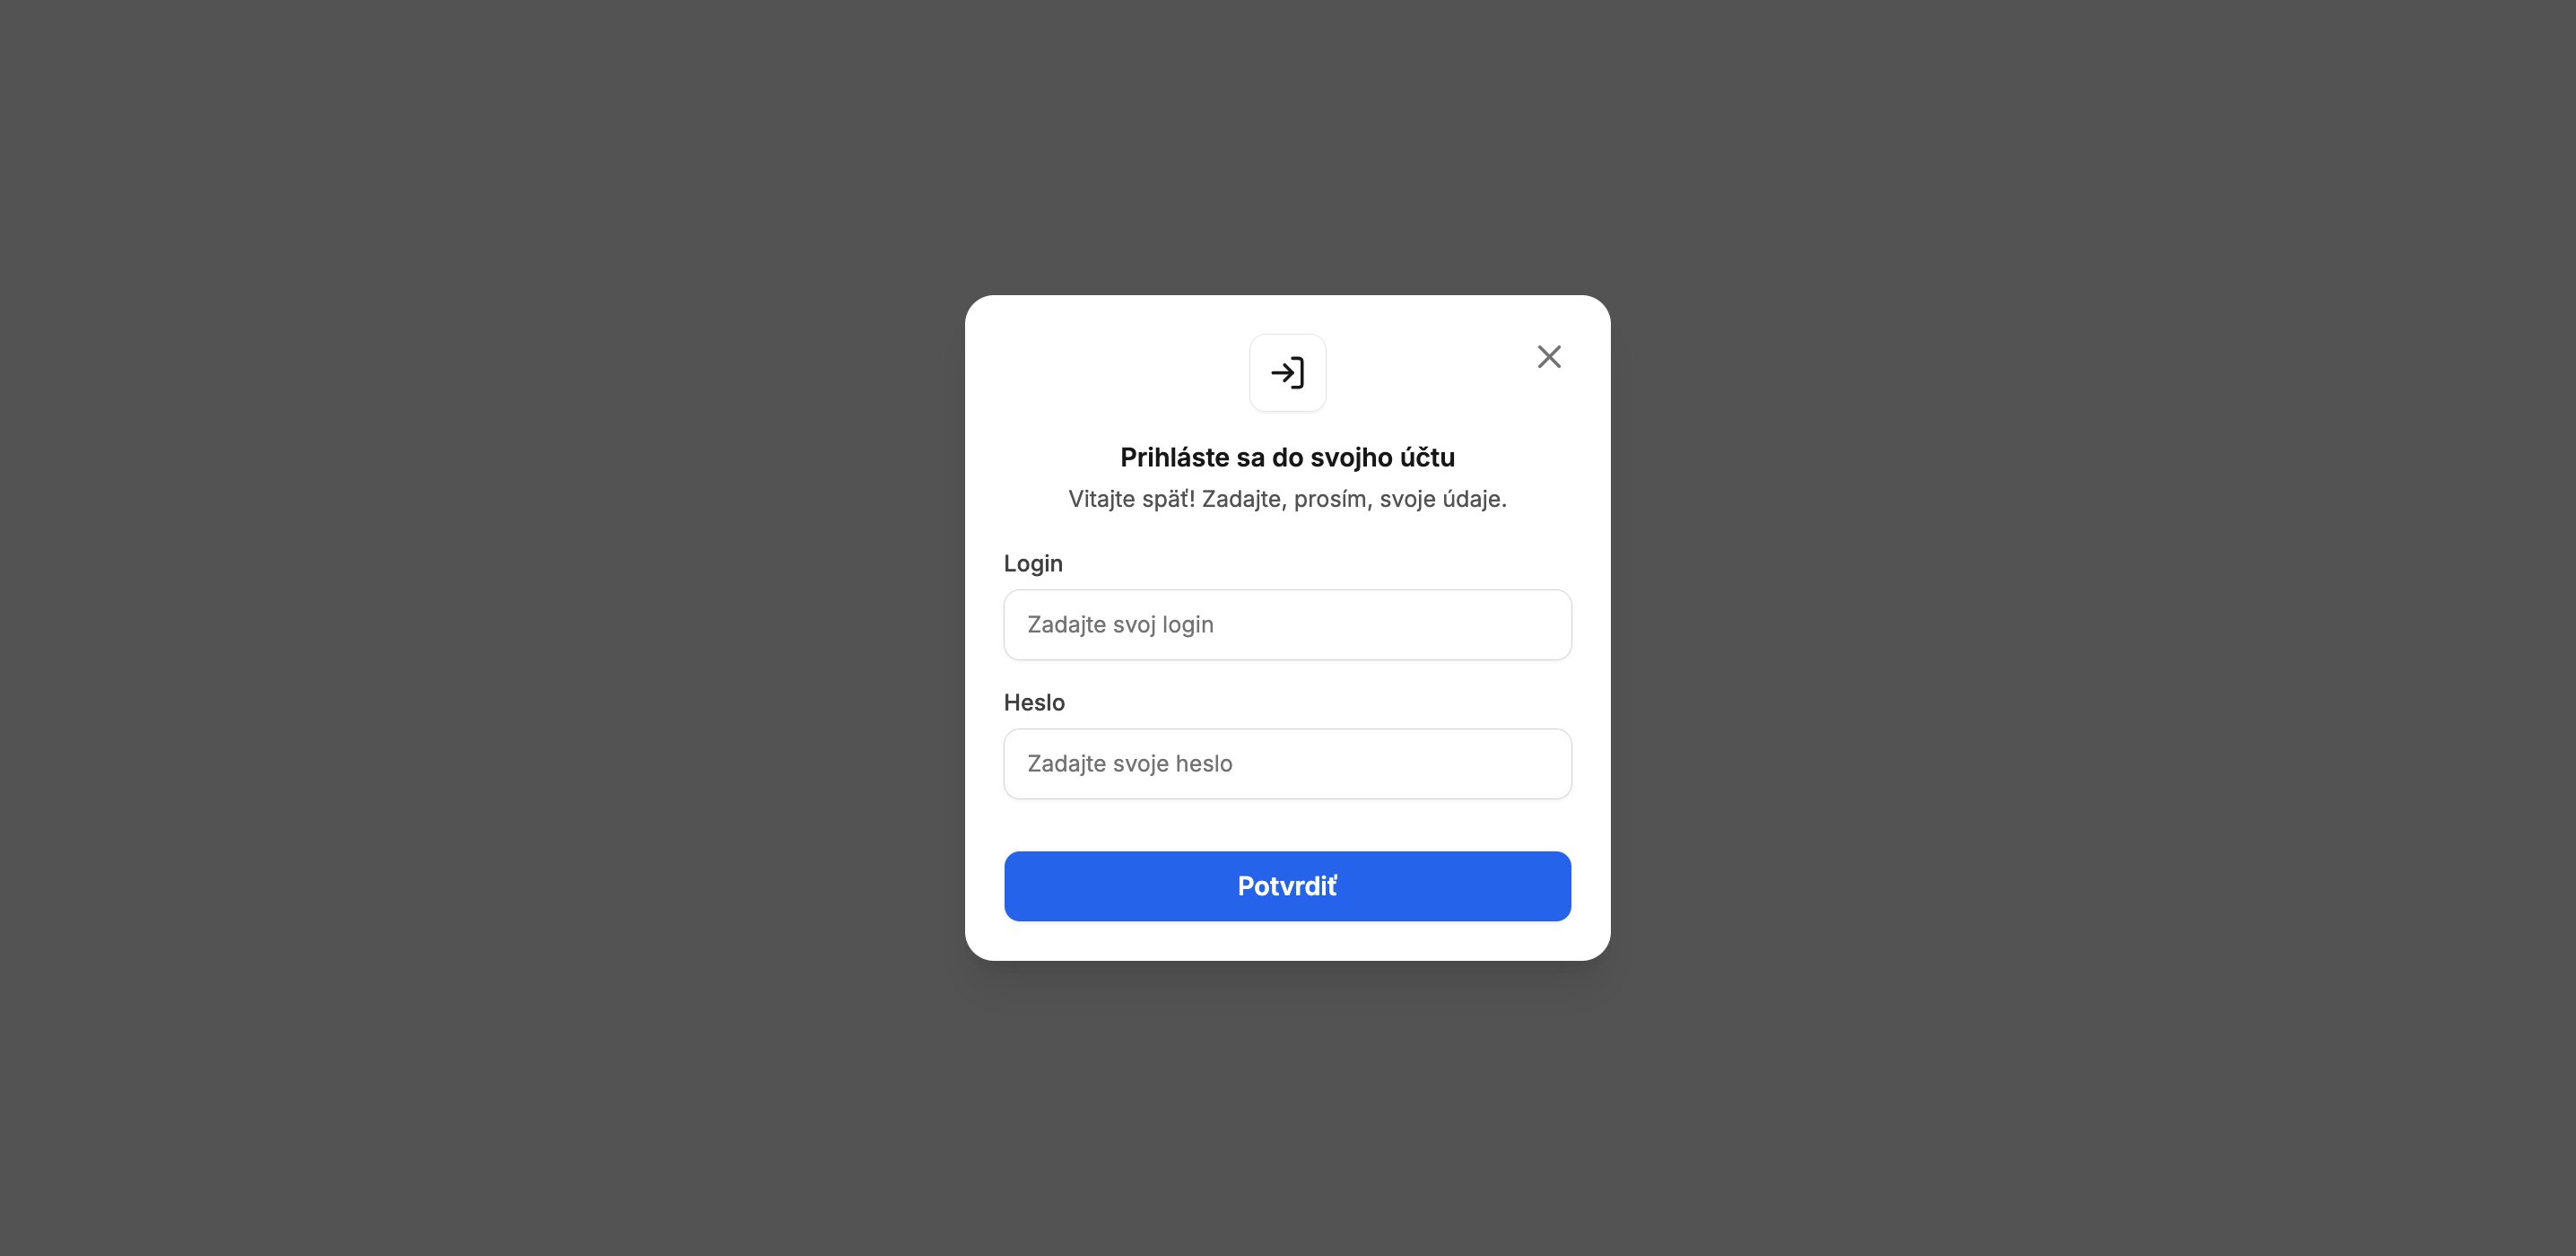
\includegraphics[width=0.72\textwidth]{figures/01-login.png}
    \caption{Prihlasovacia obrazovka frontendovej aplikácie}
\end{figure}

Ak sú prihlasovacie údaje nesprávne, používateľ zostane na rovnakej obrazovke a systém zobrazí chybové hlásenie. Po úspešnom prihlásení sa otvorí hlavná časť rozhrania dostupná pre príslušnú rolu. Navigácia je navrhnutá tak, aby sa hlavné akcie nachádzali priamo na aktuálnej obrazovke a používateľ nemusel prechádzať cez zložité menu.

\section{Administrátorské rozhranie}
\label{sec:frontend-admin}

Administrátorská časť frontendu je určená na správu učiteľských účtov a hardvérových zariadení. Po prihlásení administrátor vidí prehľadový panel so základnými štatistikami, zoznamom učiteľov a rýchlymi akciami.

\begin{figure}[!ht]
    \centering
    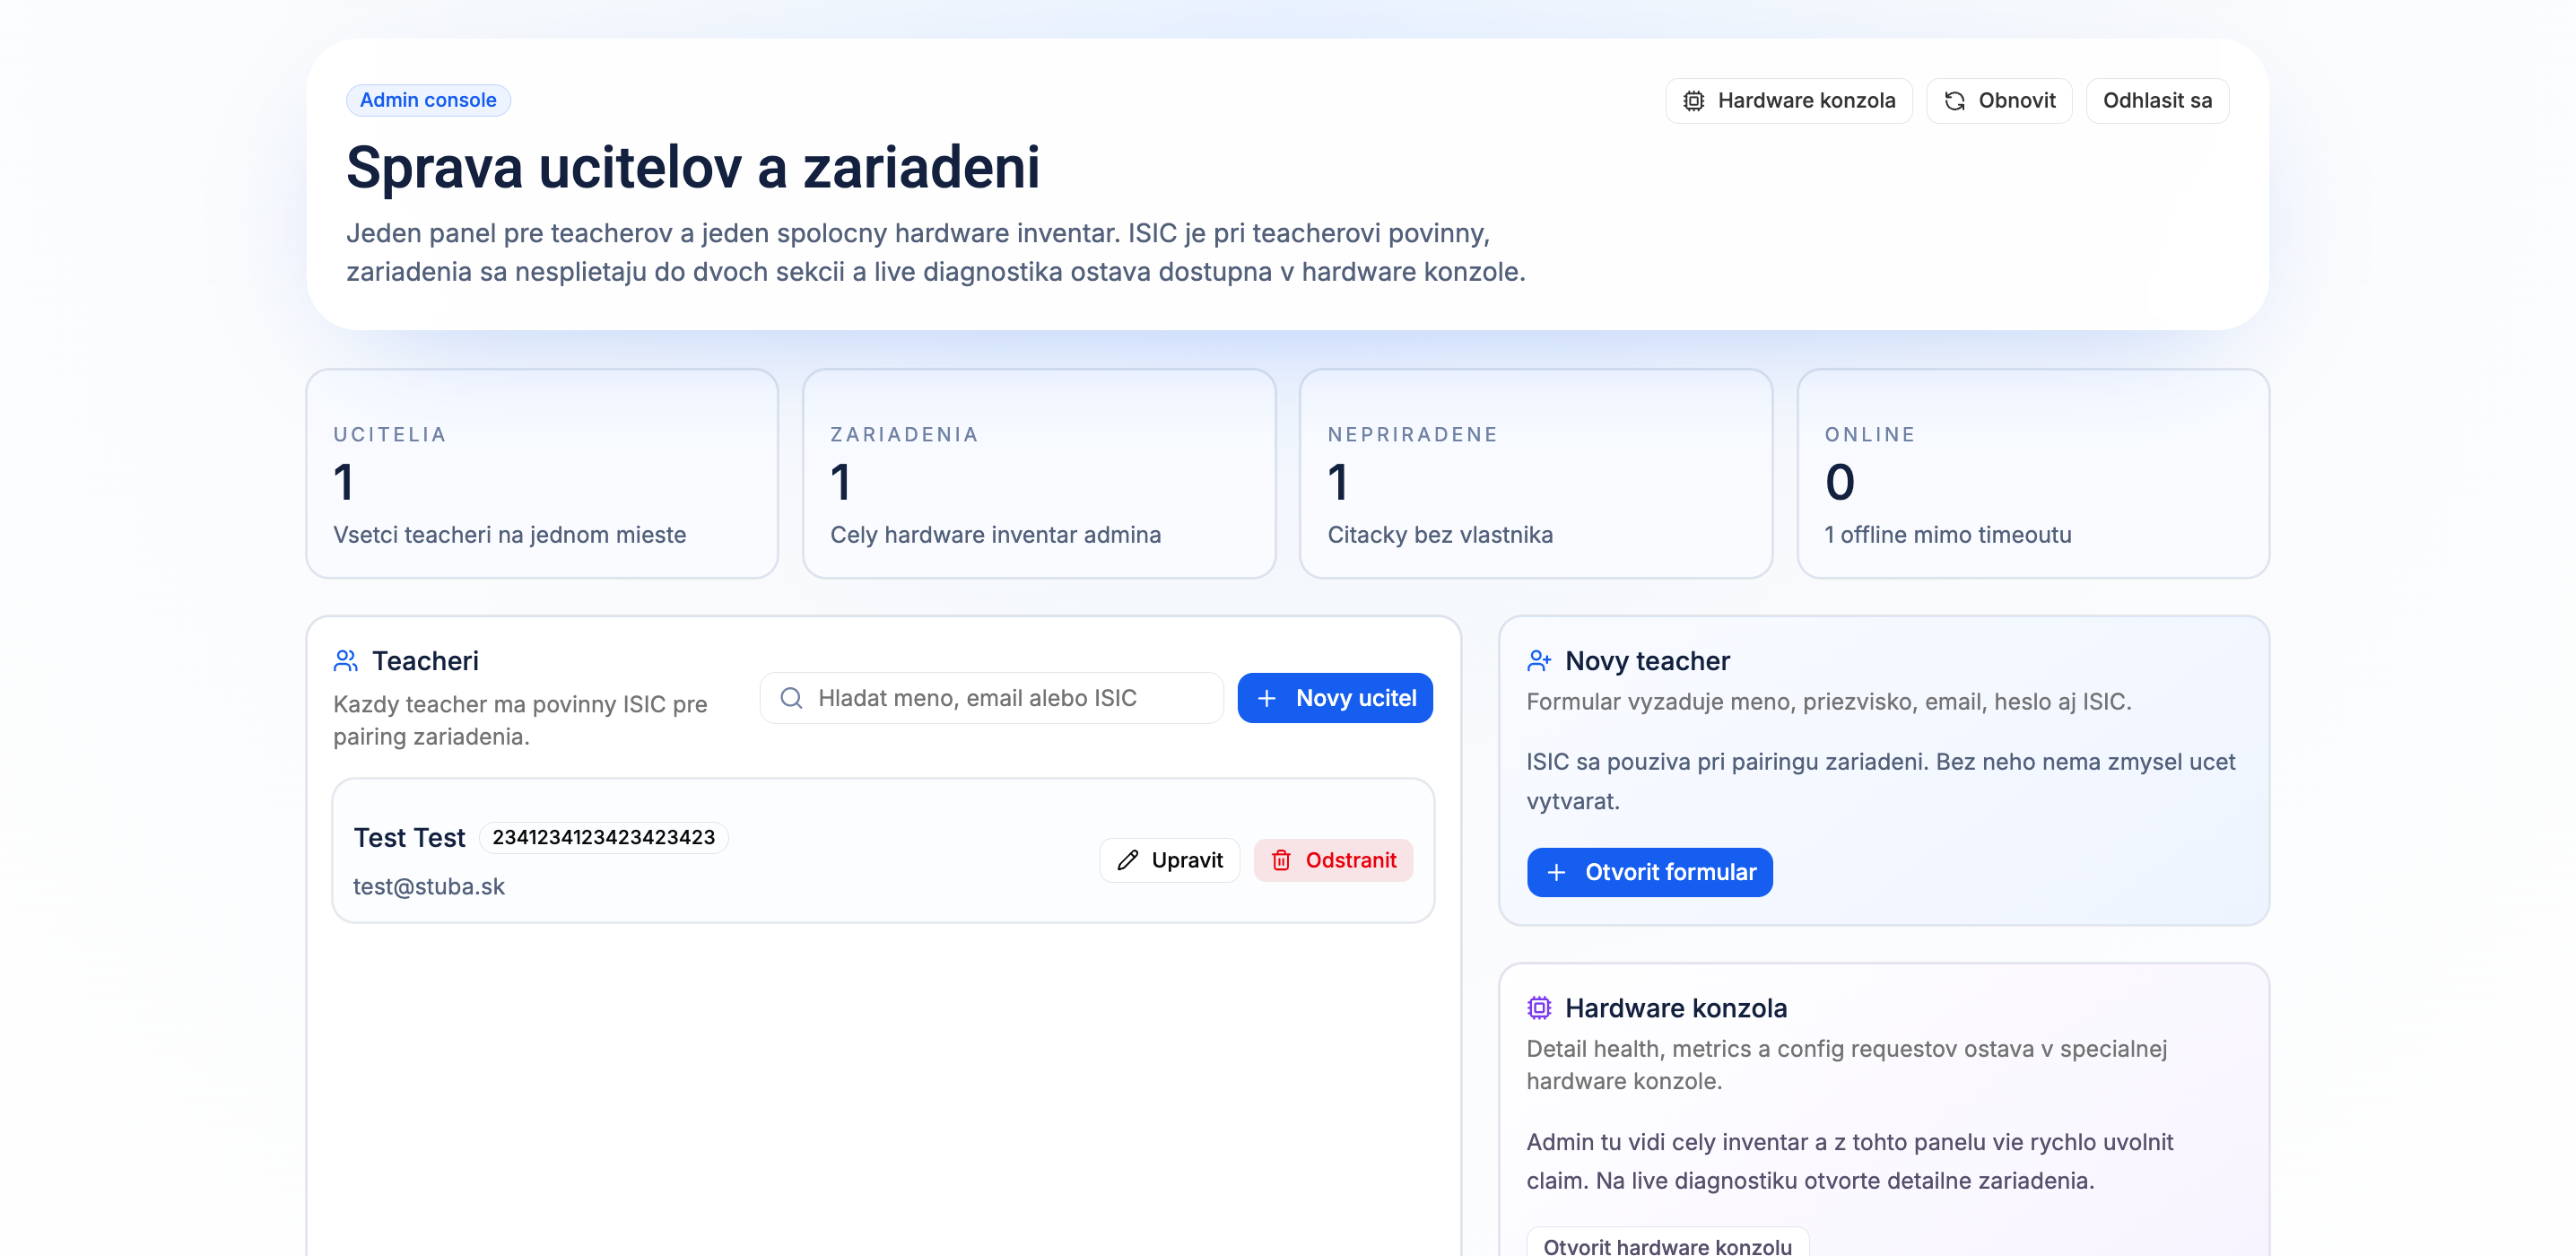
\includegraphics[width=0.95\textwidth]{figures/02-admin-dashboard.png}
    \caption{Hlavný panel administrátora}
\end{figure}

Horná časť obrazovky zobrazuje počty učiteľov, zariadení, nepriradených čítačiek a online zariadení. V zozname učiteľov je dostupné vyhľadávanie podľa mena, e-mailu alebo ISIC čísla. Tento prístup zjednodušuje správu väčšieho počtu používateľov.

Frontend obsahuje formuláre na vytvorenie, úpravu a odstránenie učiteľa. Pri vytváraní učiteľského účtu sa zadáva meno, priezvisko, e-mail, heslo a ISIC číslo. Pri úprave zostávajú povinné identifikačné údaje, pričom zmena hesla je voliteľná.

\begin{figure}[!ht]
    \centering
    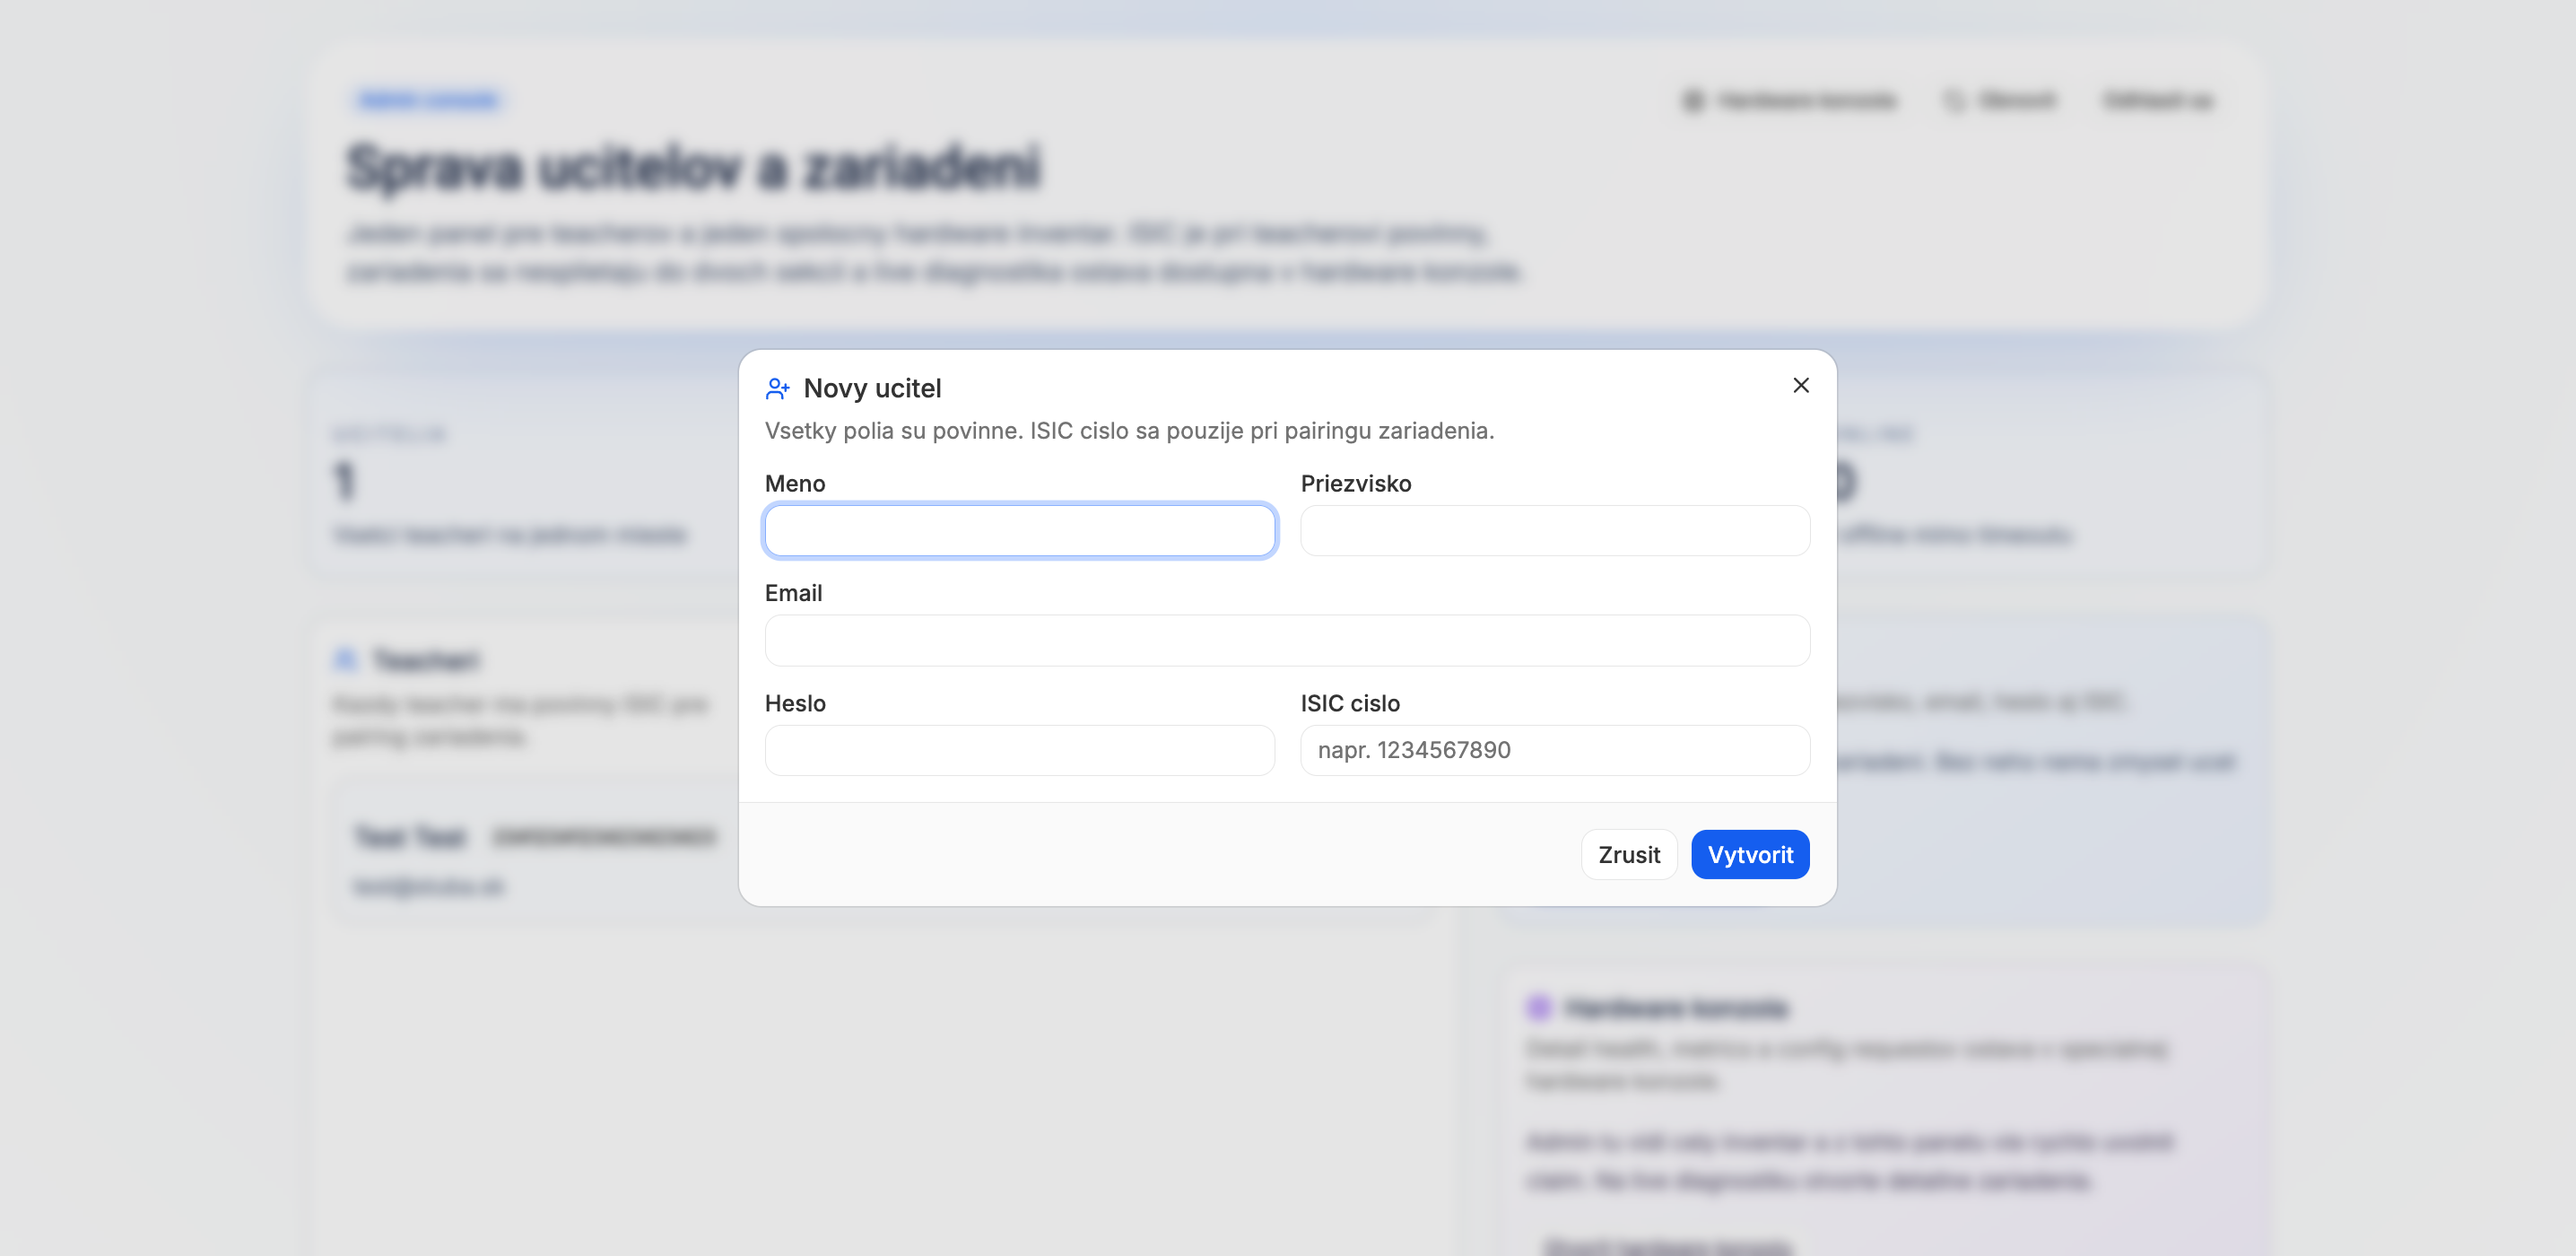
\includegraphics[width=0.82\textwidth]{figures/03-admin-new-teacher.png}
    \caption{Formulár na vytvorenie nového učiteľa}
\end{figure}

Odstránenie účtu je chránené potvrdzovacím dialógom. Tým sa znižuje riziko náhodného zmazania používateľa. Dôležitou súčasťou administrátorského rozhrania je aj hardvérová konzola, v ktorej možno filtrovať zariadenia podľa stavu a otvoriť detail konkrétnej čítačky.

\begin{figure}[!ht]
    \centering
    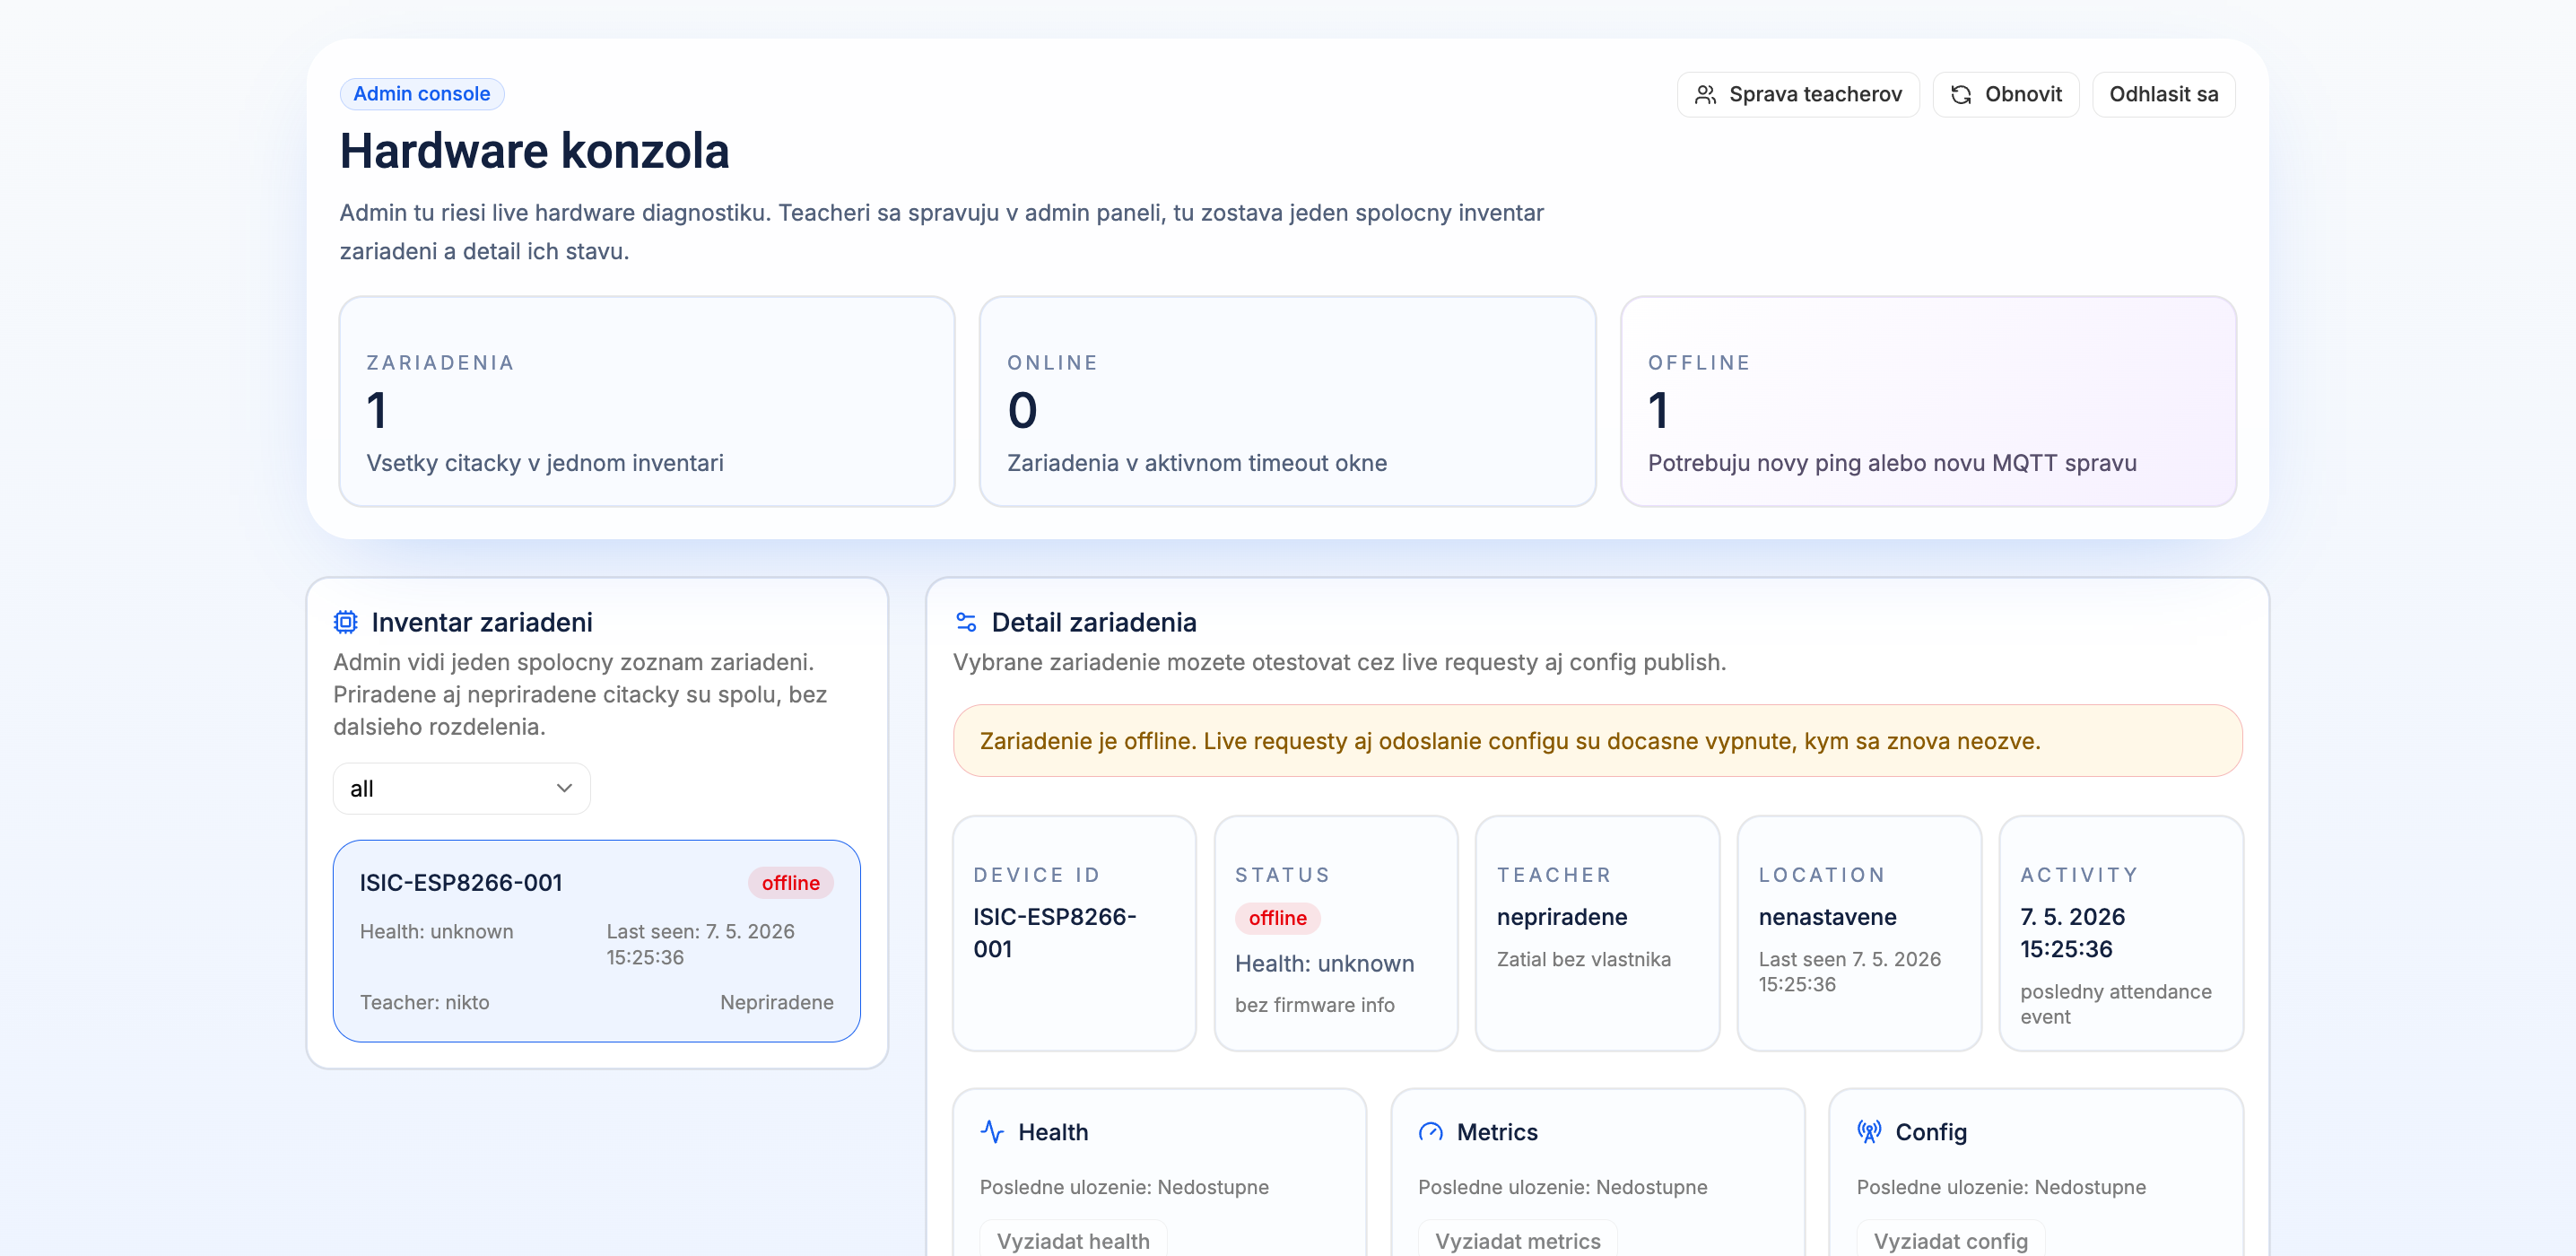
\includegraphics[width=0.92\textwidth]{figures/07-admin-hardware-detail.png}
    \caption{Detail hardvérového zariadenia v administrátorskom rozhraní}
\end{figure}

V detaile zariadenia frontend zobrazuje identifikátor zariadenia, online stav, health stav, priradeného učiteľa, lokáciu a poslednú aktivitu. Rozhranie zároveň umožňuje vyžiadať health údaje, zobraziť metriky a upraviť konfiguračný JSON. Takéto riešenie zjednocuje správu používateľov aj hardvéru do jedného webového rozhrania.

\section{Rozhranie vyučujúceho}
\label{sec:frontend-teacher}

Rozhranie vyučujúceho je zamerané najmä na prácu so semestrom, týždňami, rozvrhovými jednotkami a dochádzkou. Po prihlásení sa zobrazí týždenný kalendár s bočným panelom týždňov a horným panelom akcií.

\begin{figure}[!ht]
    \centering
    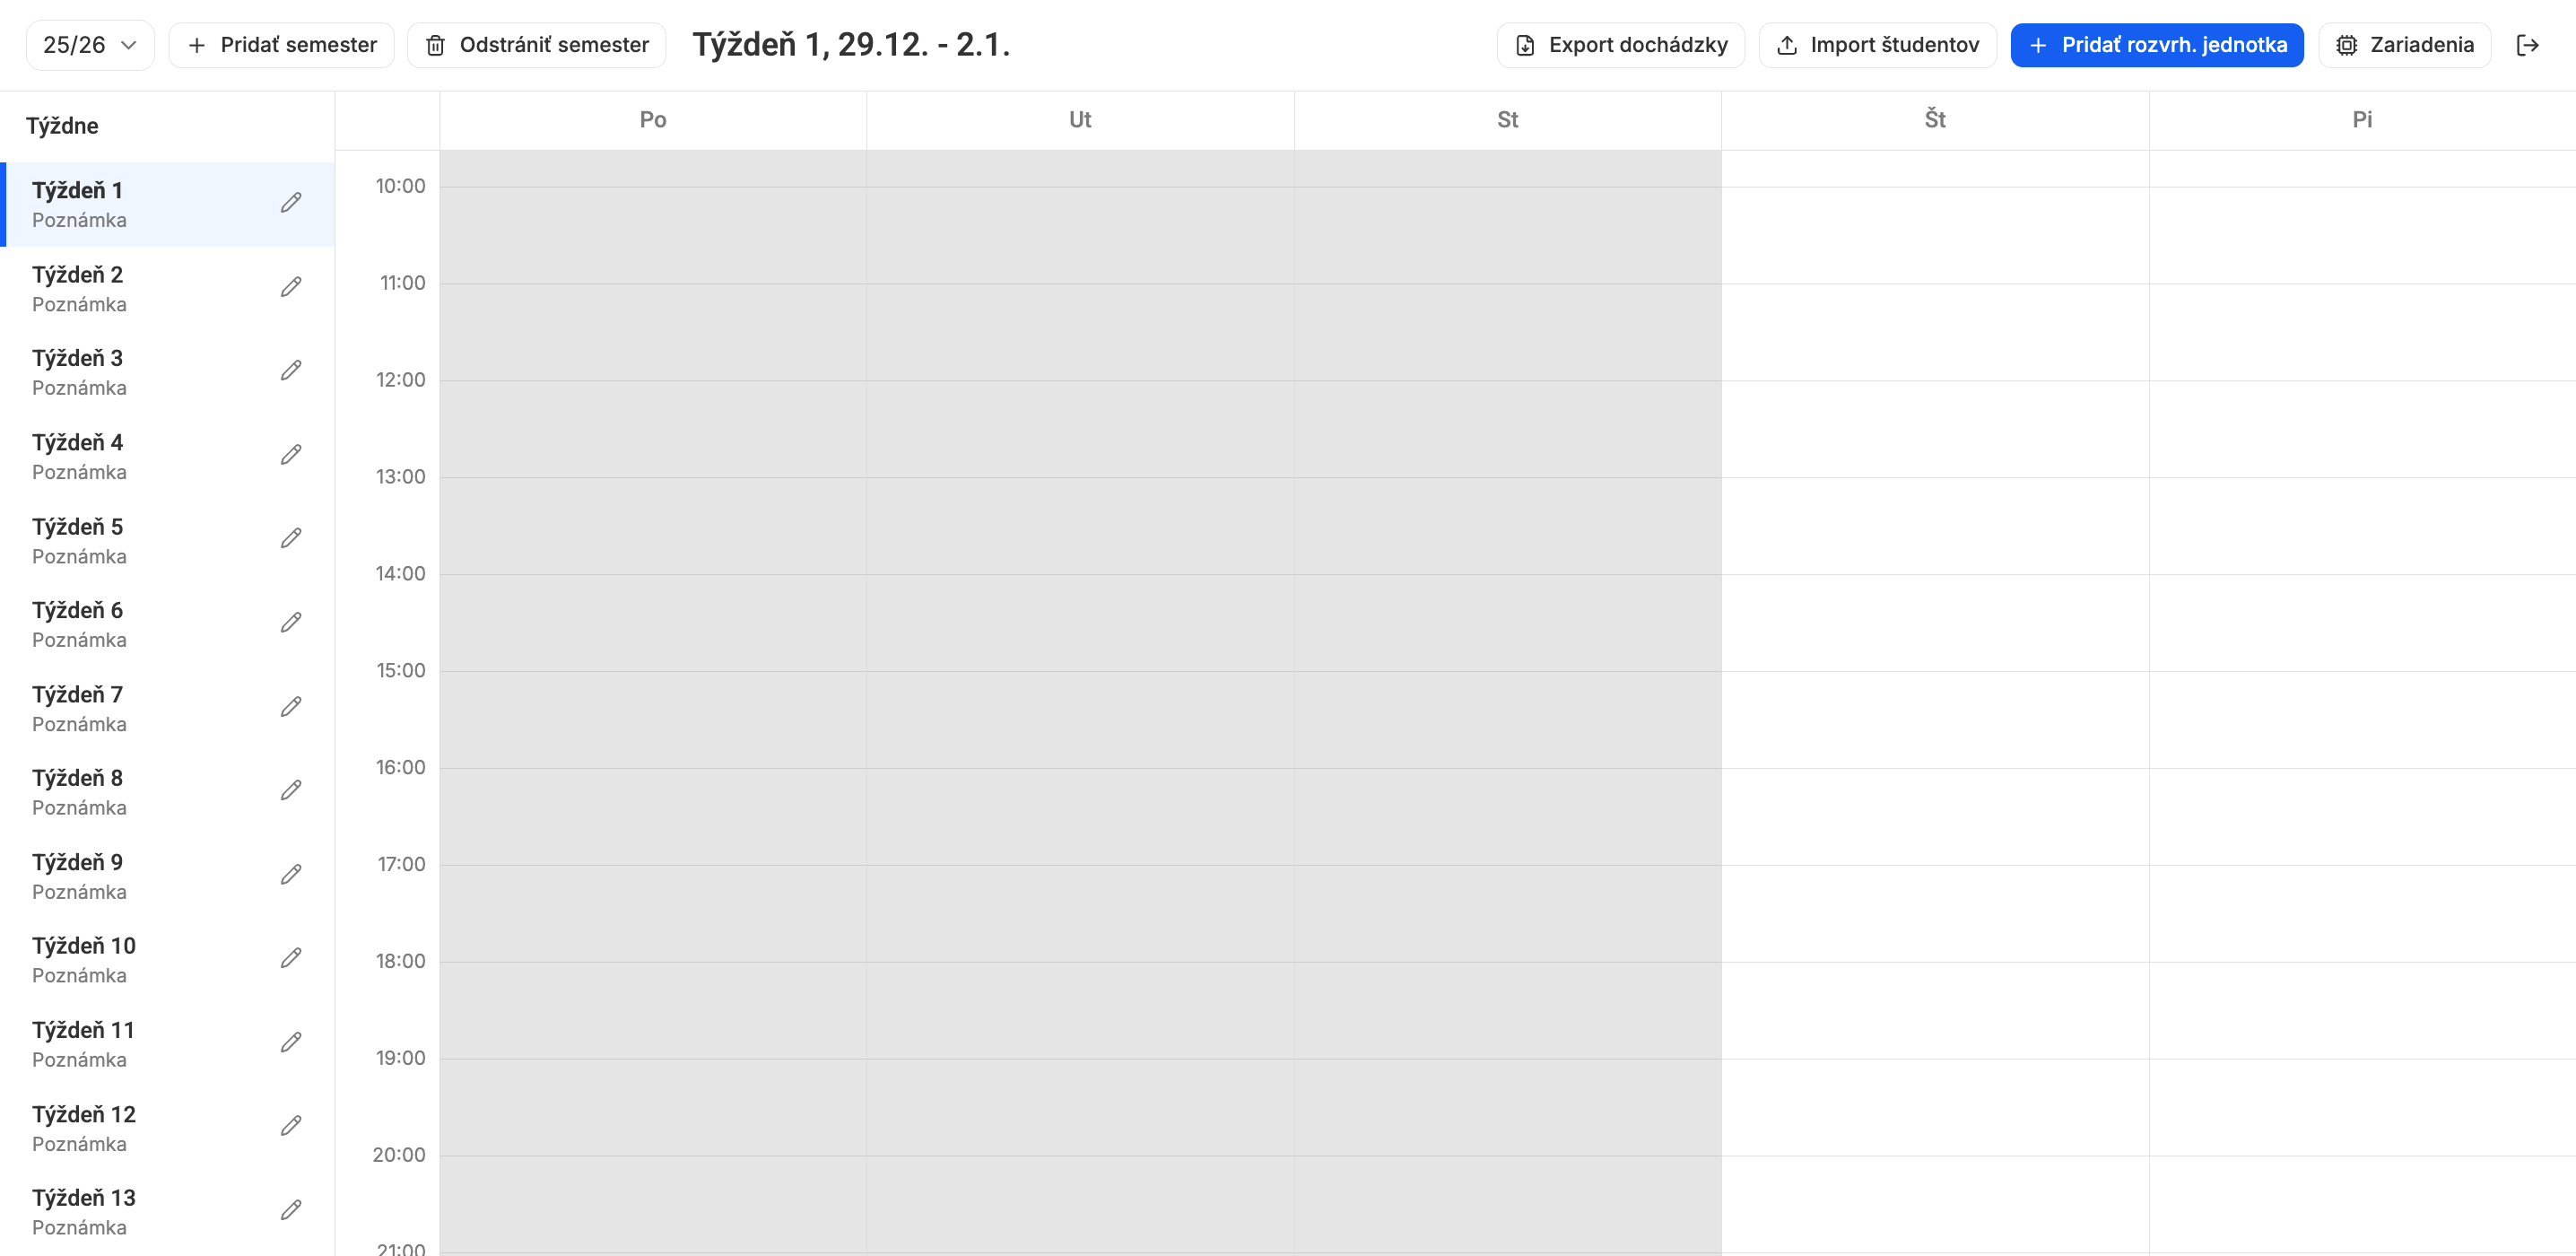
\includegraphics[width=0.95\textwidth]{figures/08-teacher-calendar.png}
    \caption{Kalendárové rozhranie vyučujúceho}
\end{figure}

Horný panel umožňuje vybrať semester, vytvoriť nový semester, odstrániť aktuálny semester, importovať študentov, exportovať dochádzku a pridať novú rozvrhovú jednotku. V ľavej časti sa nachádza zoznam týždňov semestra. Kliknutím na týždeň sa načítajú hodiny a príslušná dochádzka pre zvolený interval.

Vytvorenie nového semestra prebieha cez samostatný dialóg. Používateľ zadá názov semestra, dátum začiatku a počet týždňov. Frontend následne odošle údaje backendu a po úspešnom vytvorení automaticky obnoví zobrazenie.

\begin{figure}[!ht]
    \centering
    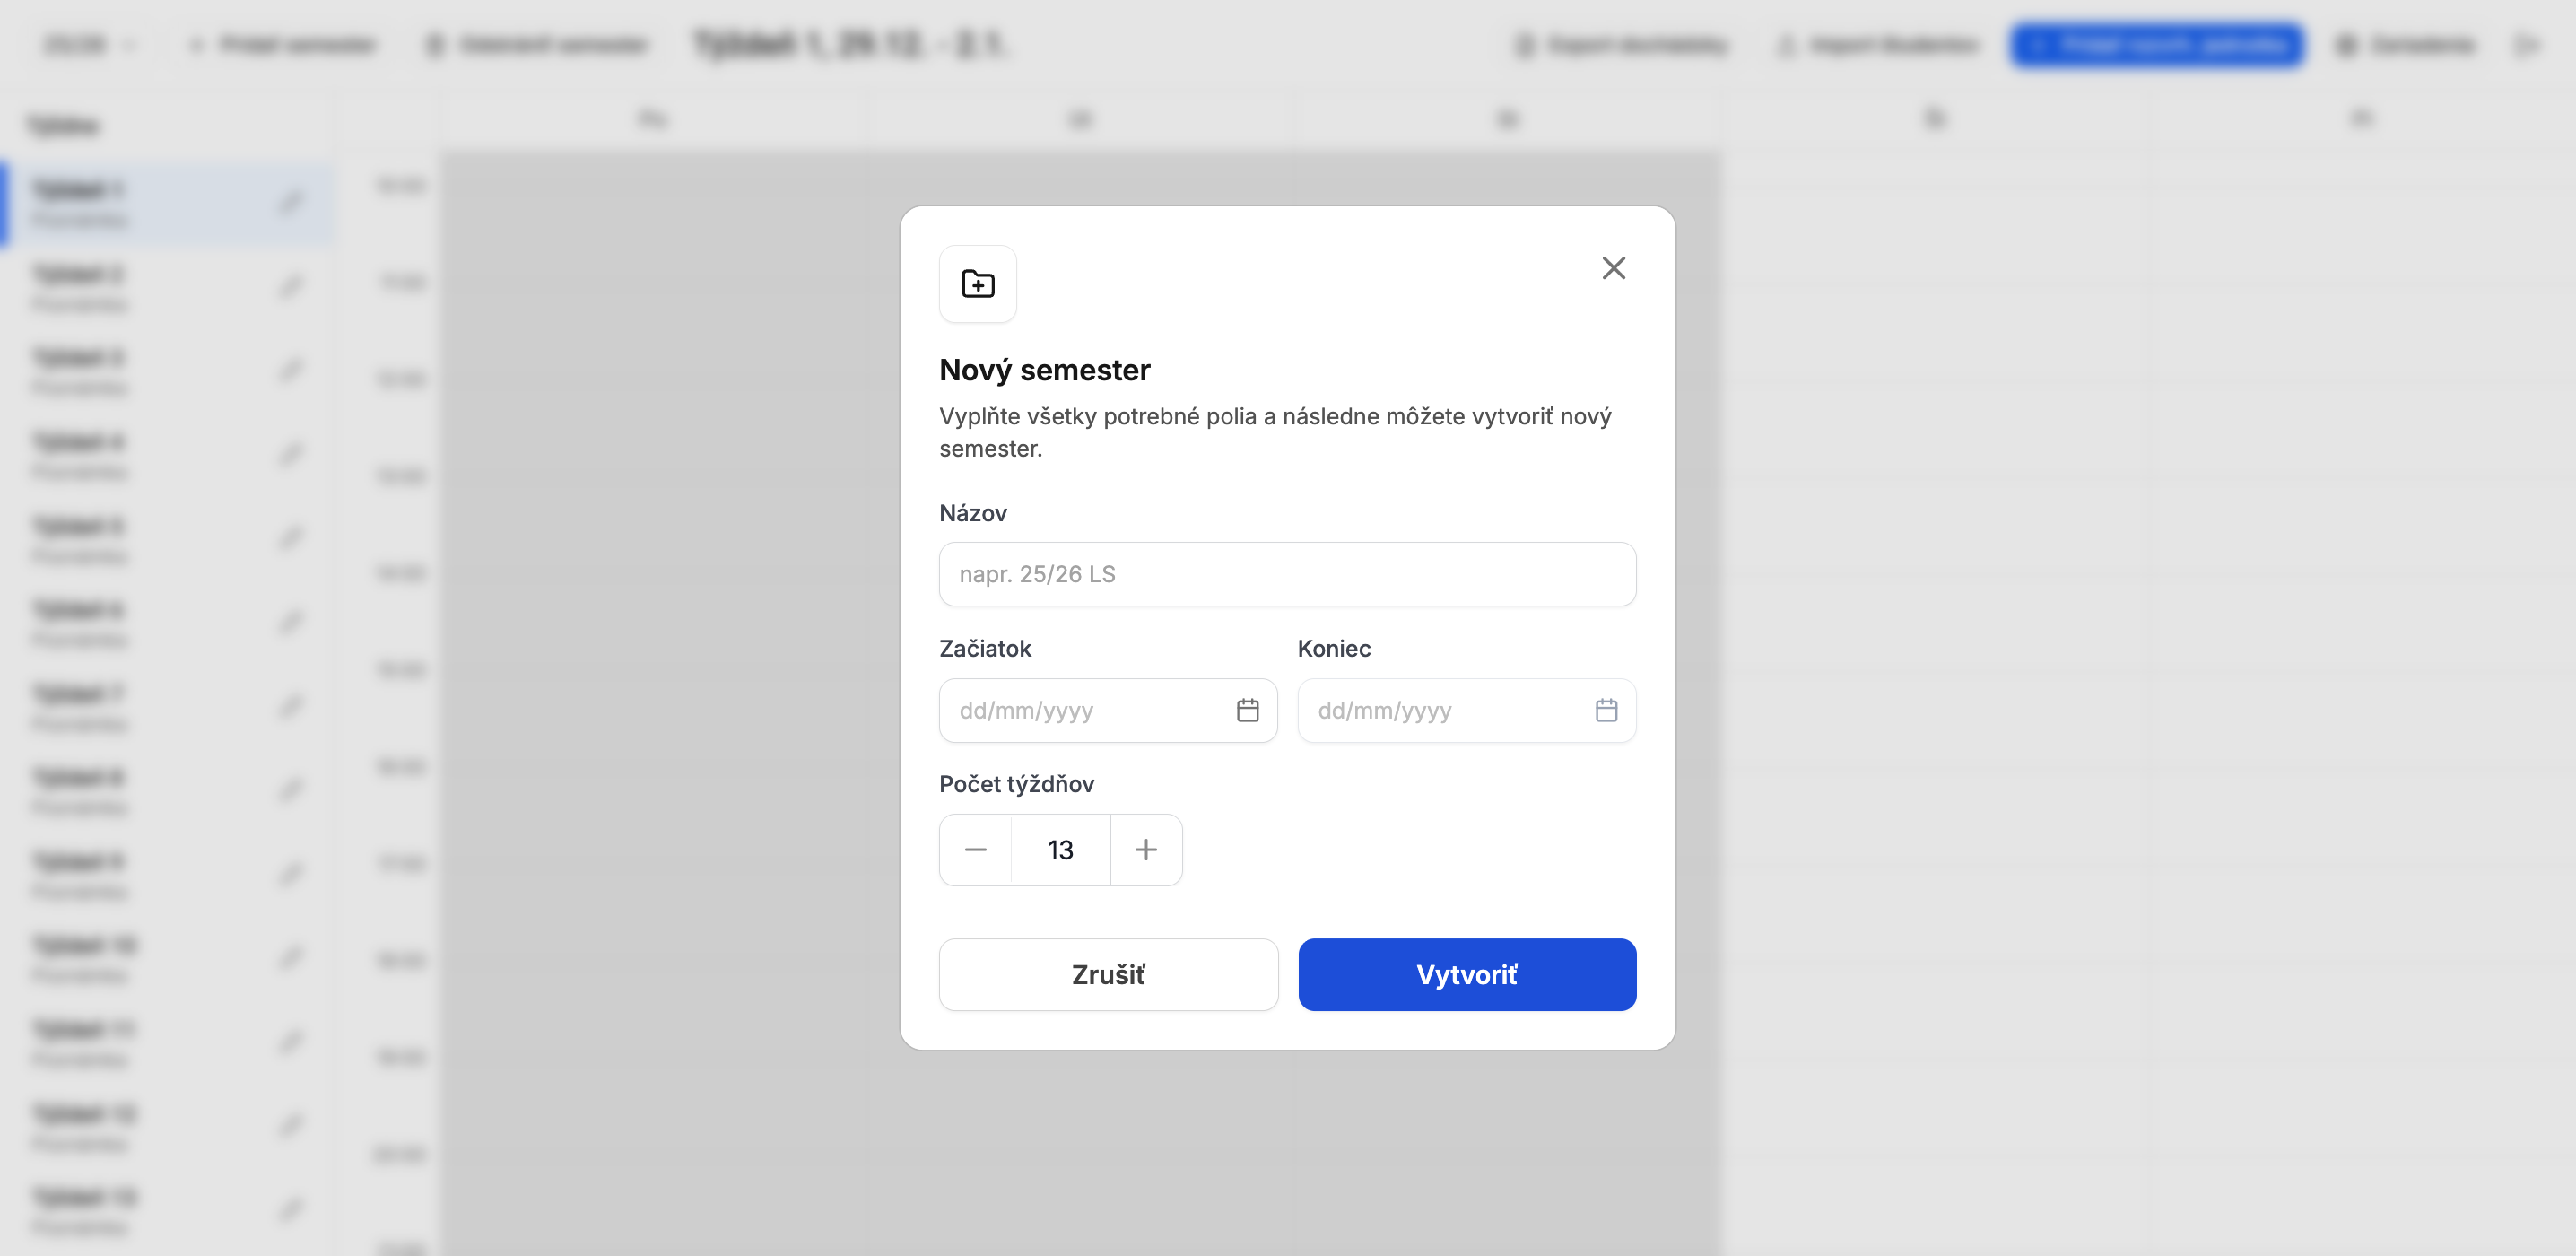
\includegraphics[width=0.76\textwidth]{figures/09-teacher-new-semester.png}
    \caption{Dialóg na vytvorenie nového semestra}
\end{figure}

Rozvrhové jednotky možno vytvárať ako opakujúce sa alebo jednorazové udalosti. Formulár obsahuje názov predmetu, typ hodiny, čas začiatku a konca, miestnosť, farebné odlíšenie a pravidlá opakovania.

\begin{figure}[!ht]
    \centering
    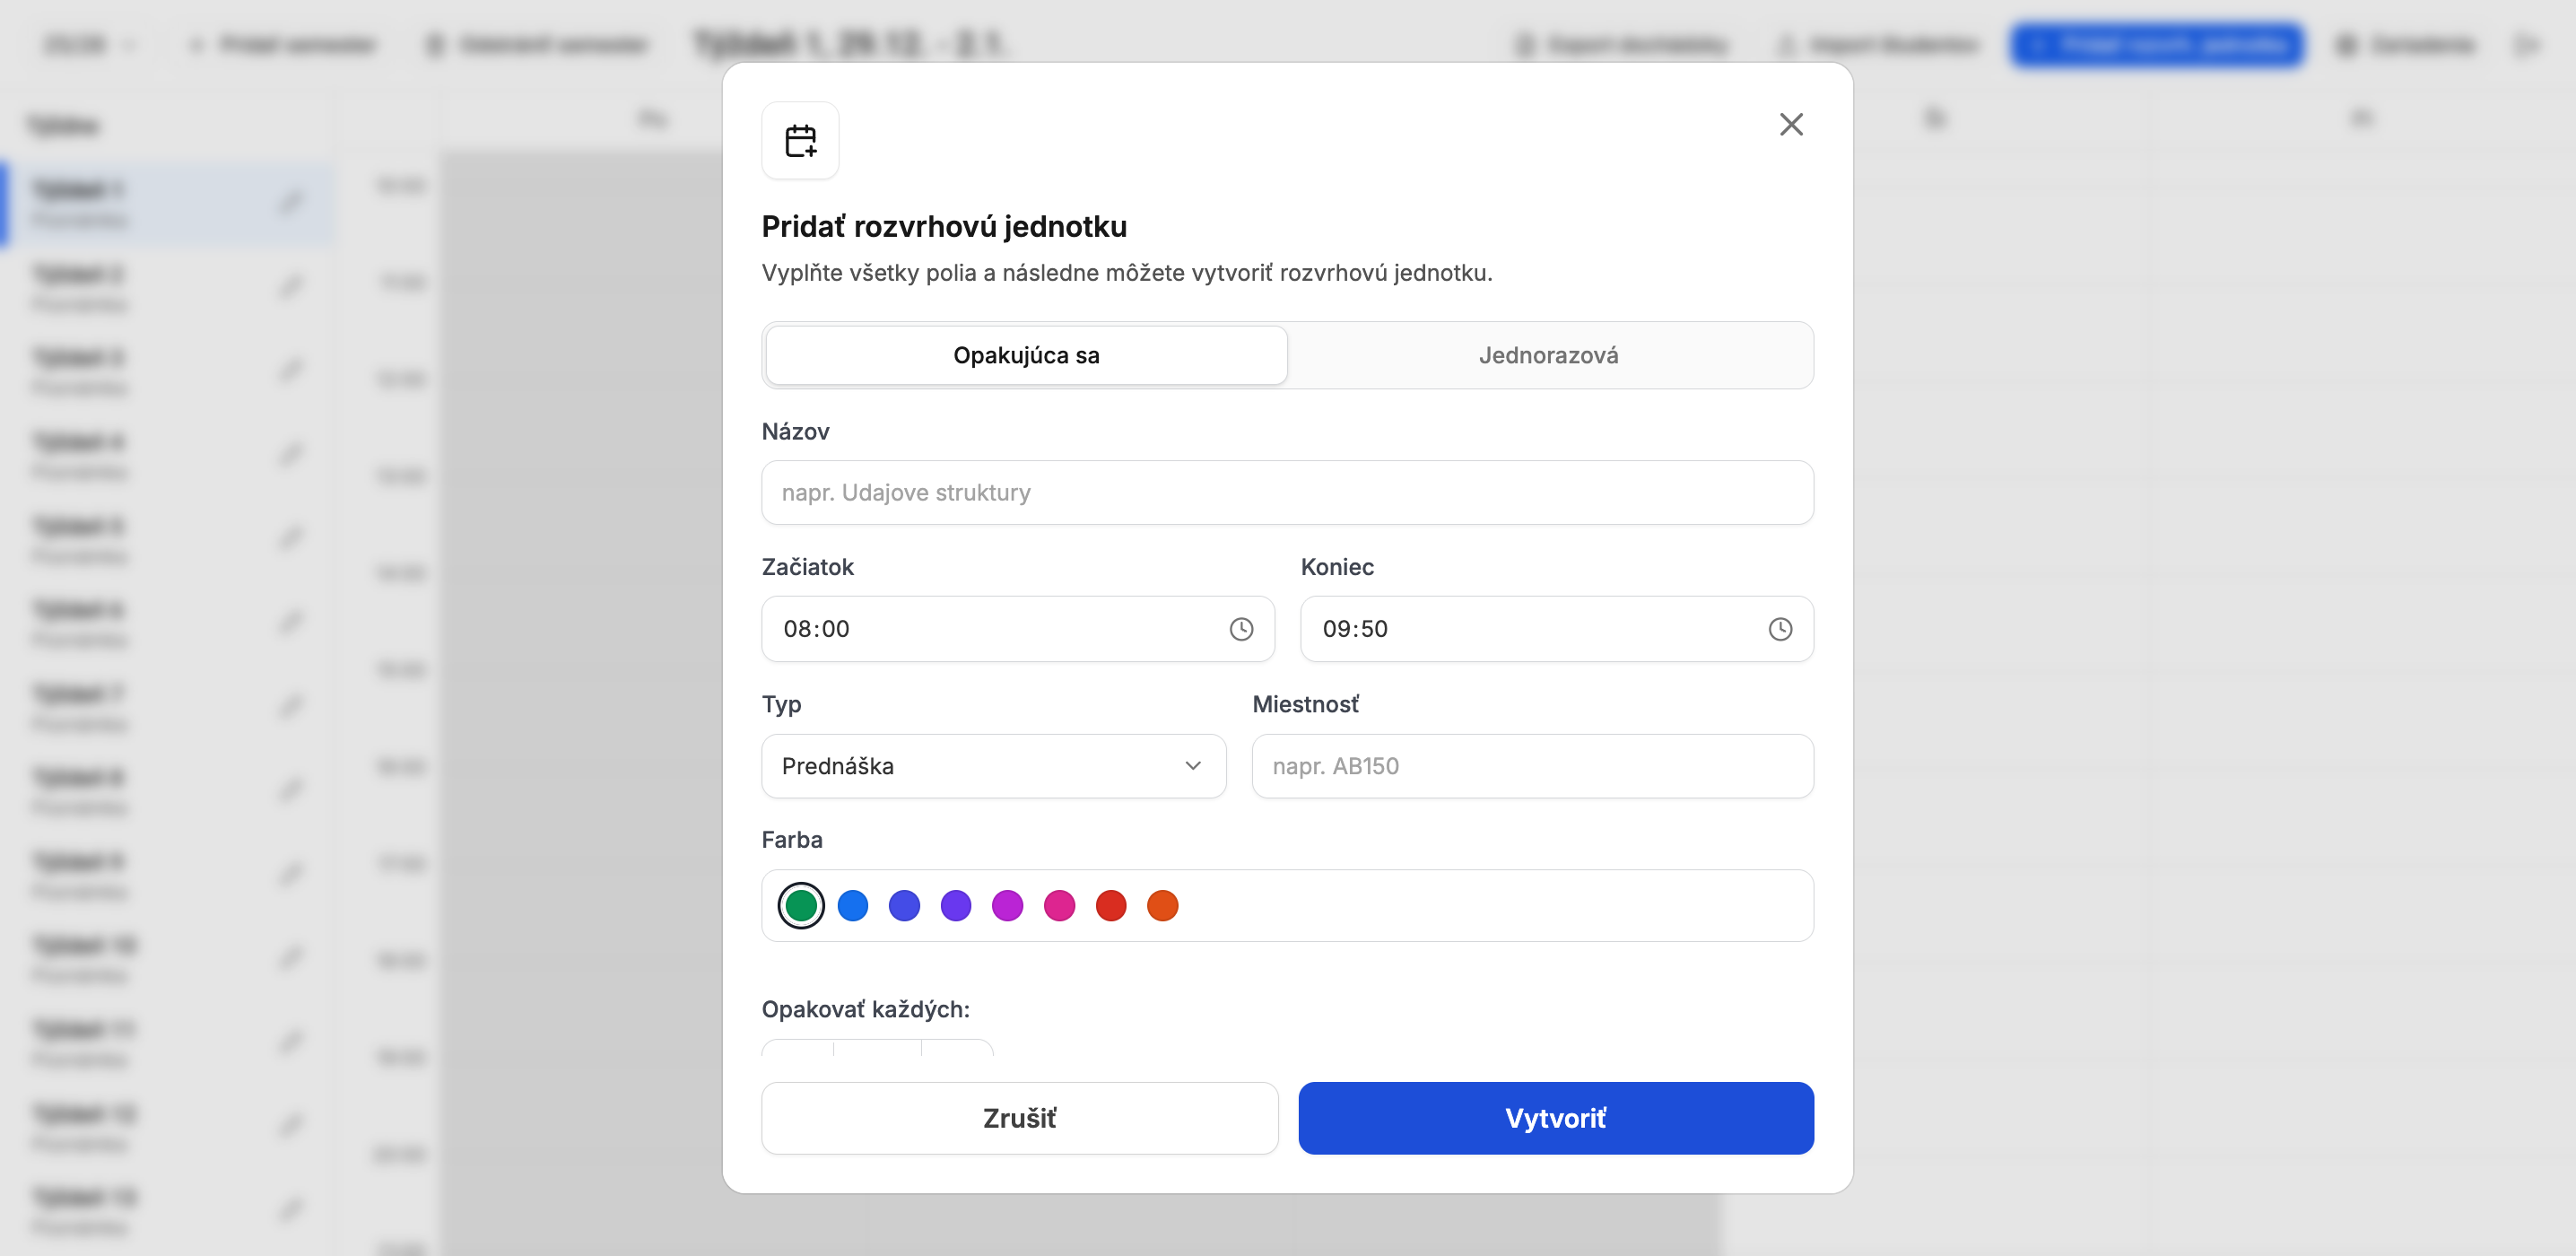
\includegraphics[width=0.78\textwidth]{figures/10-teacher-schedule-entry.png}
    \caption{Formulár na vytvorenie rozvrhovej jednotky}
\end{figure}

Po vytvorení sa rozvrhová jednotka zobrazí priamo v časovej mriežke kalendára. Kliknutie na konkrétnu hodinu otvorí detail udalosti so zoznamom študentov a ich aktuálnou dochádzkou.

\section{Import, export a správa dochádzky}
\label{sec:frontend-attendance}

Frontend poskytuje samostatné dialógy na import študentov a export dochádzky. Pri importe používateľ najskôr vyberie predmet a potom nahrá CSV súbor. Rozhranie zobrazuje aj náhľad prvých riadkov súboru, čím pomáha odhaliť chybný formát ešte pred samotným odoslaním na backend.

\begin{figure}[!ht]
    \centering
    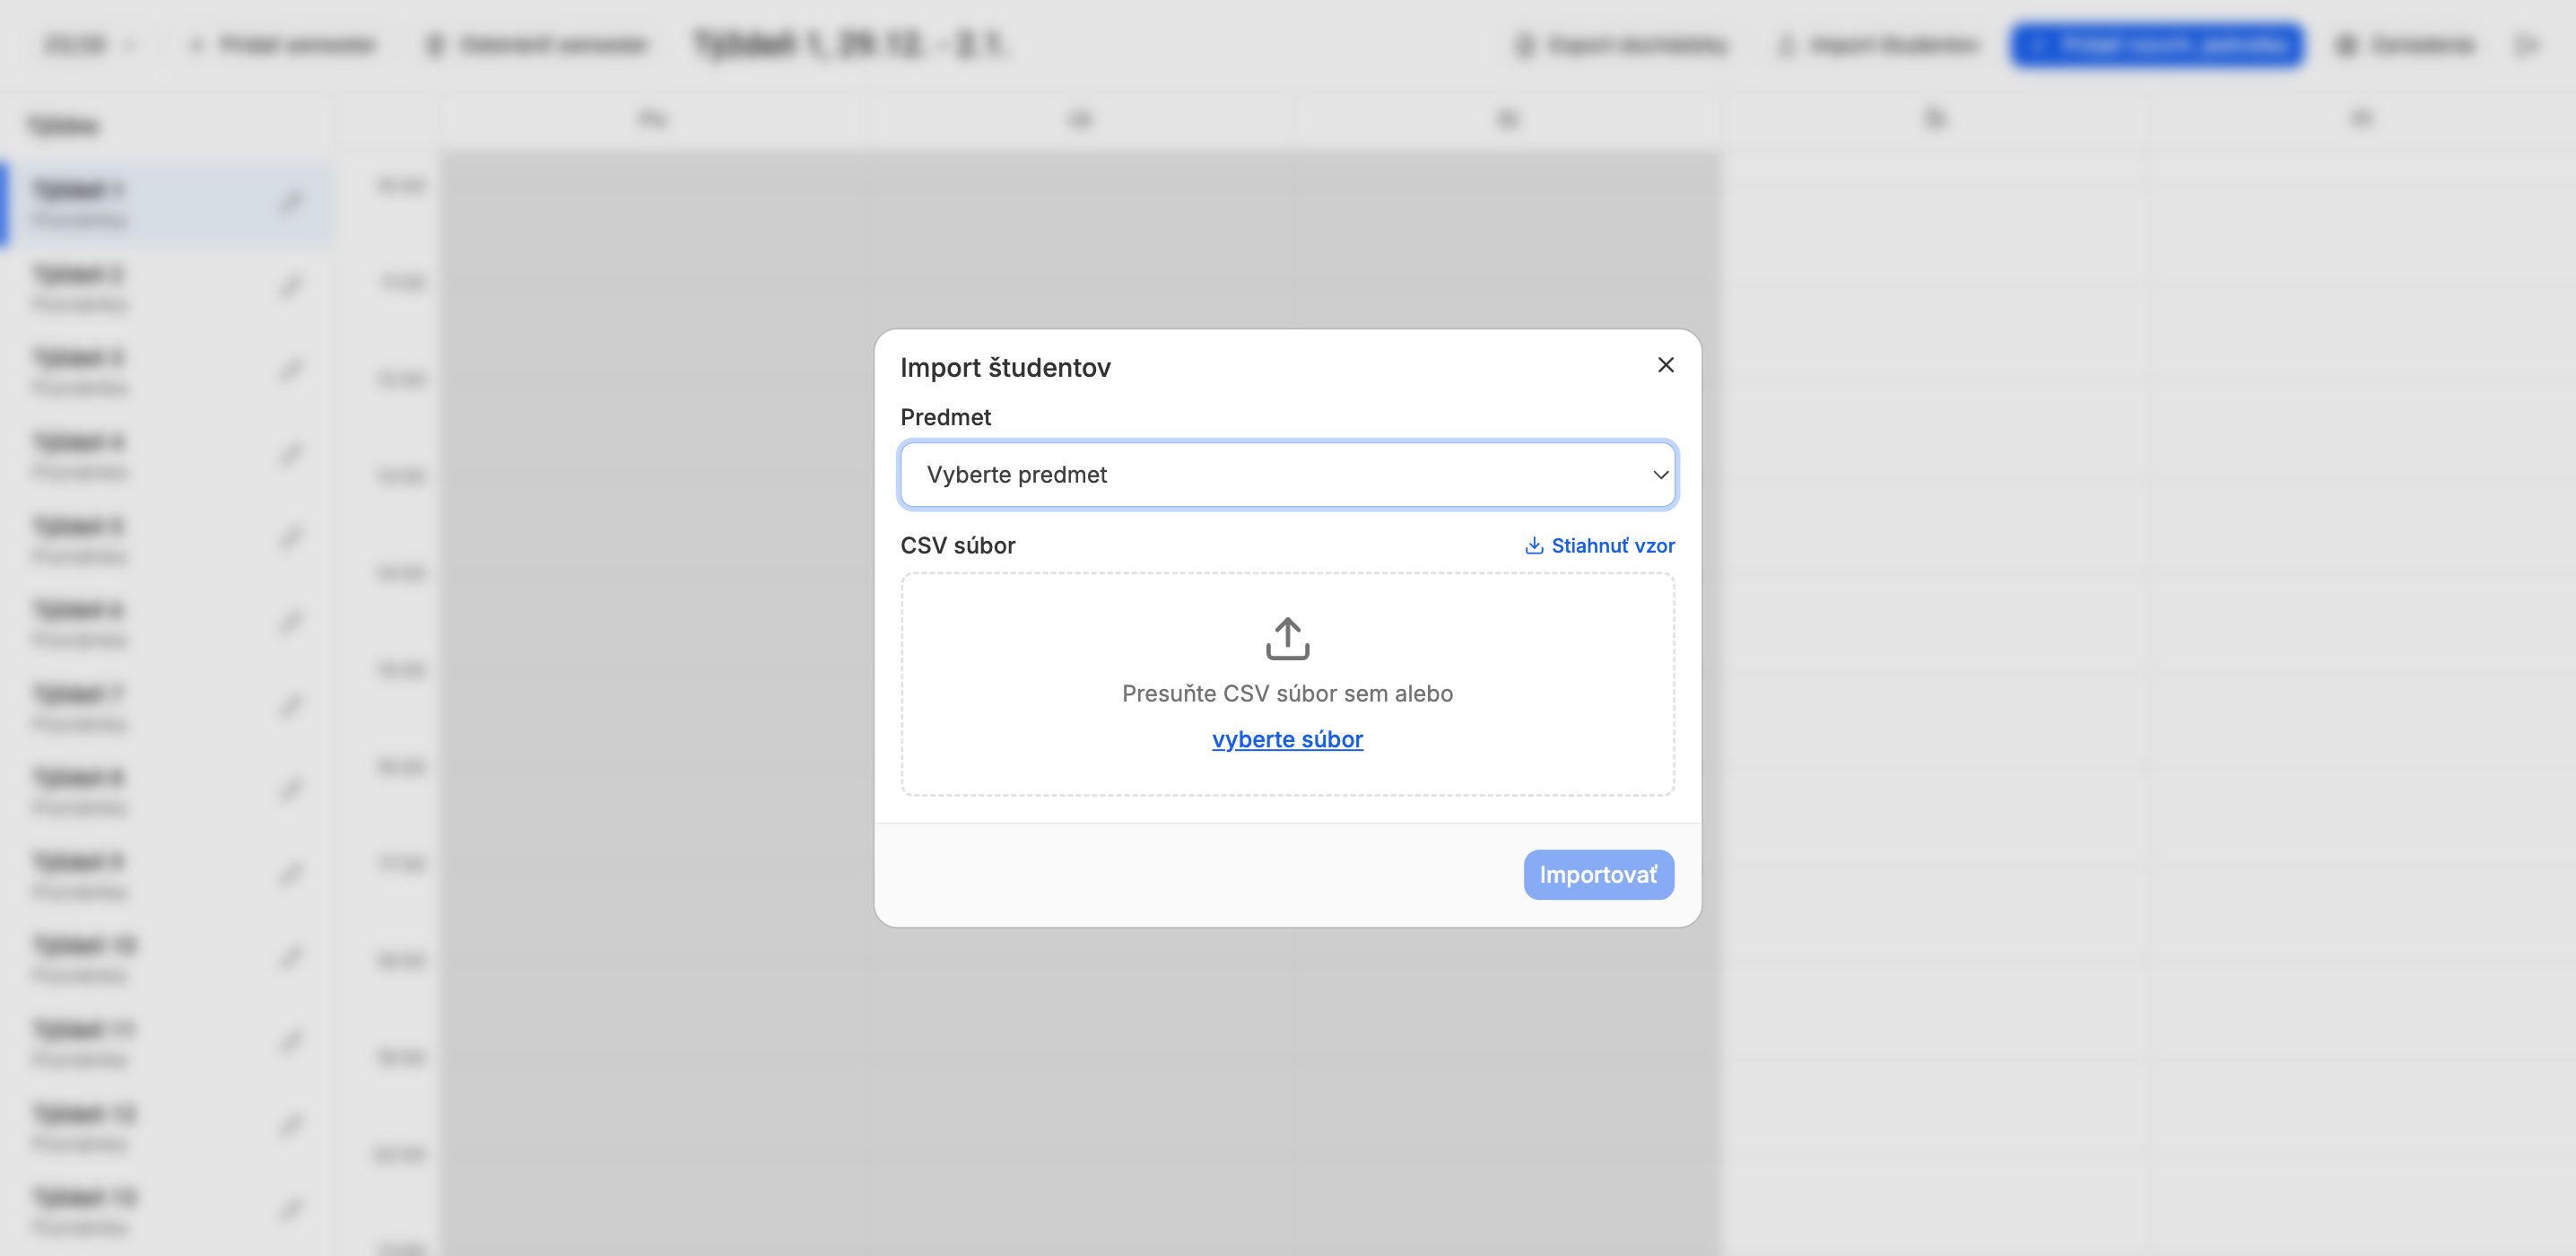
\includegraphics[width=0.82\textwidth]{figures/11-teacher-import-students.png}
    \caption{Dialóg na import študentov z CSV súboru}
\end{figure}

Pri exporte si vyučujúci vyberie predmet a frontend následne stiahne výsledný súbor z backendu. Export je určený najmä na ďalšie spracovanie dochádzky mimo samotnej aplikácie.

\begin{figure}[!ht]
    \centering
    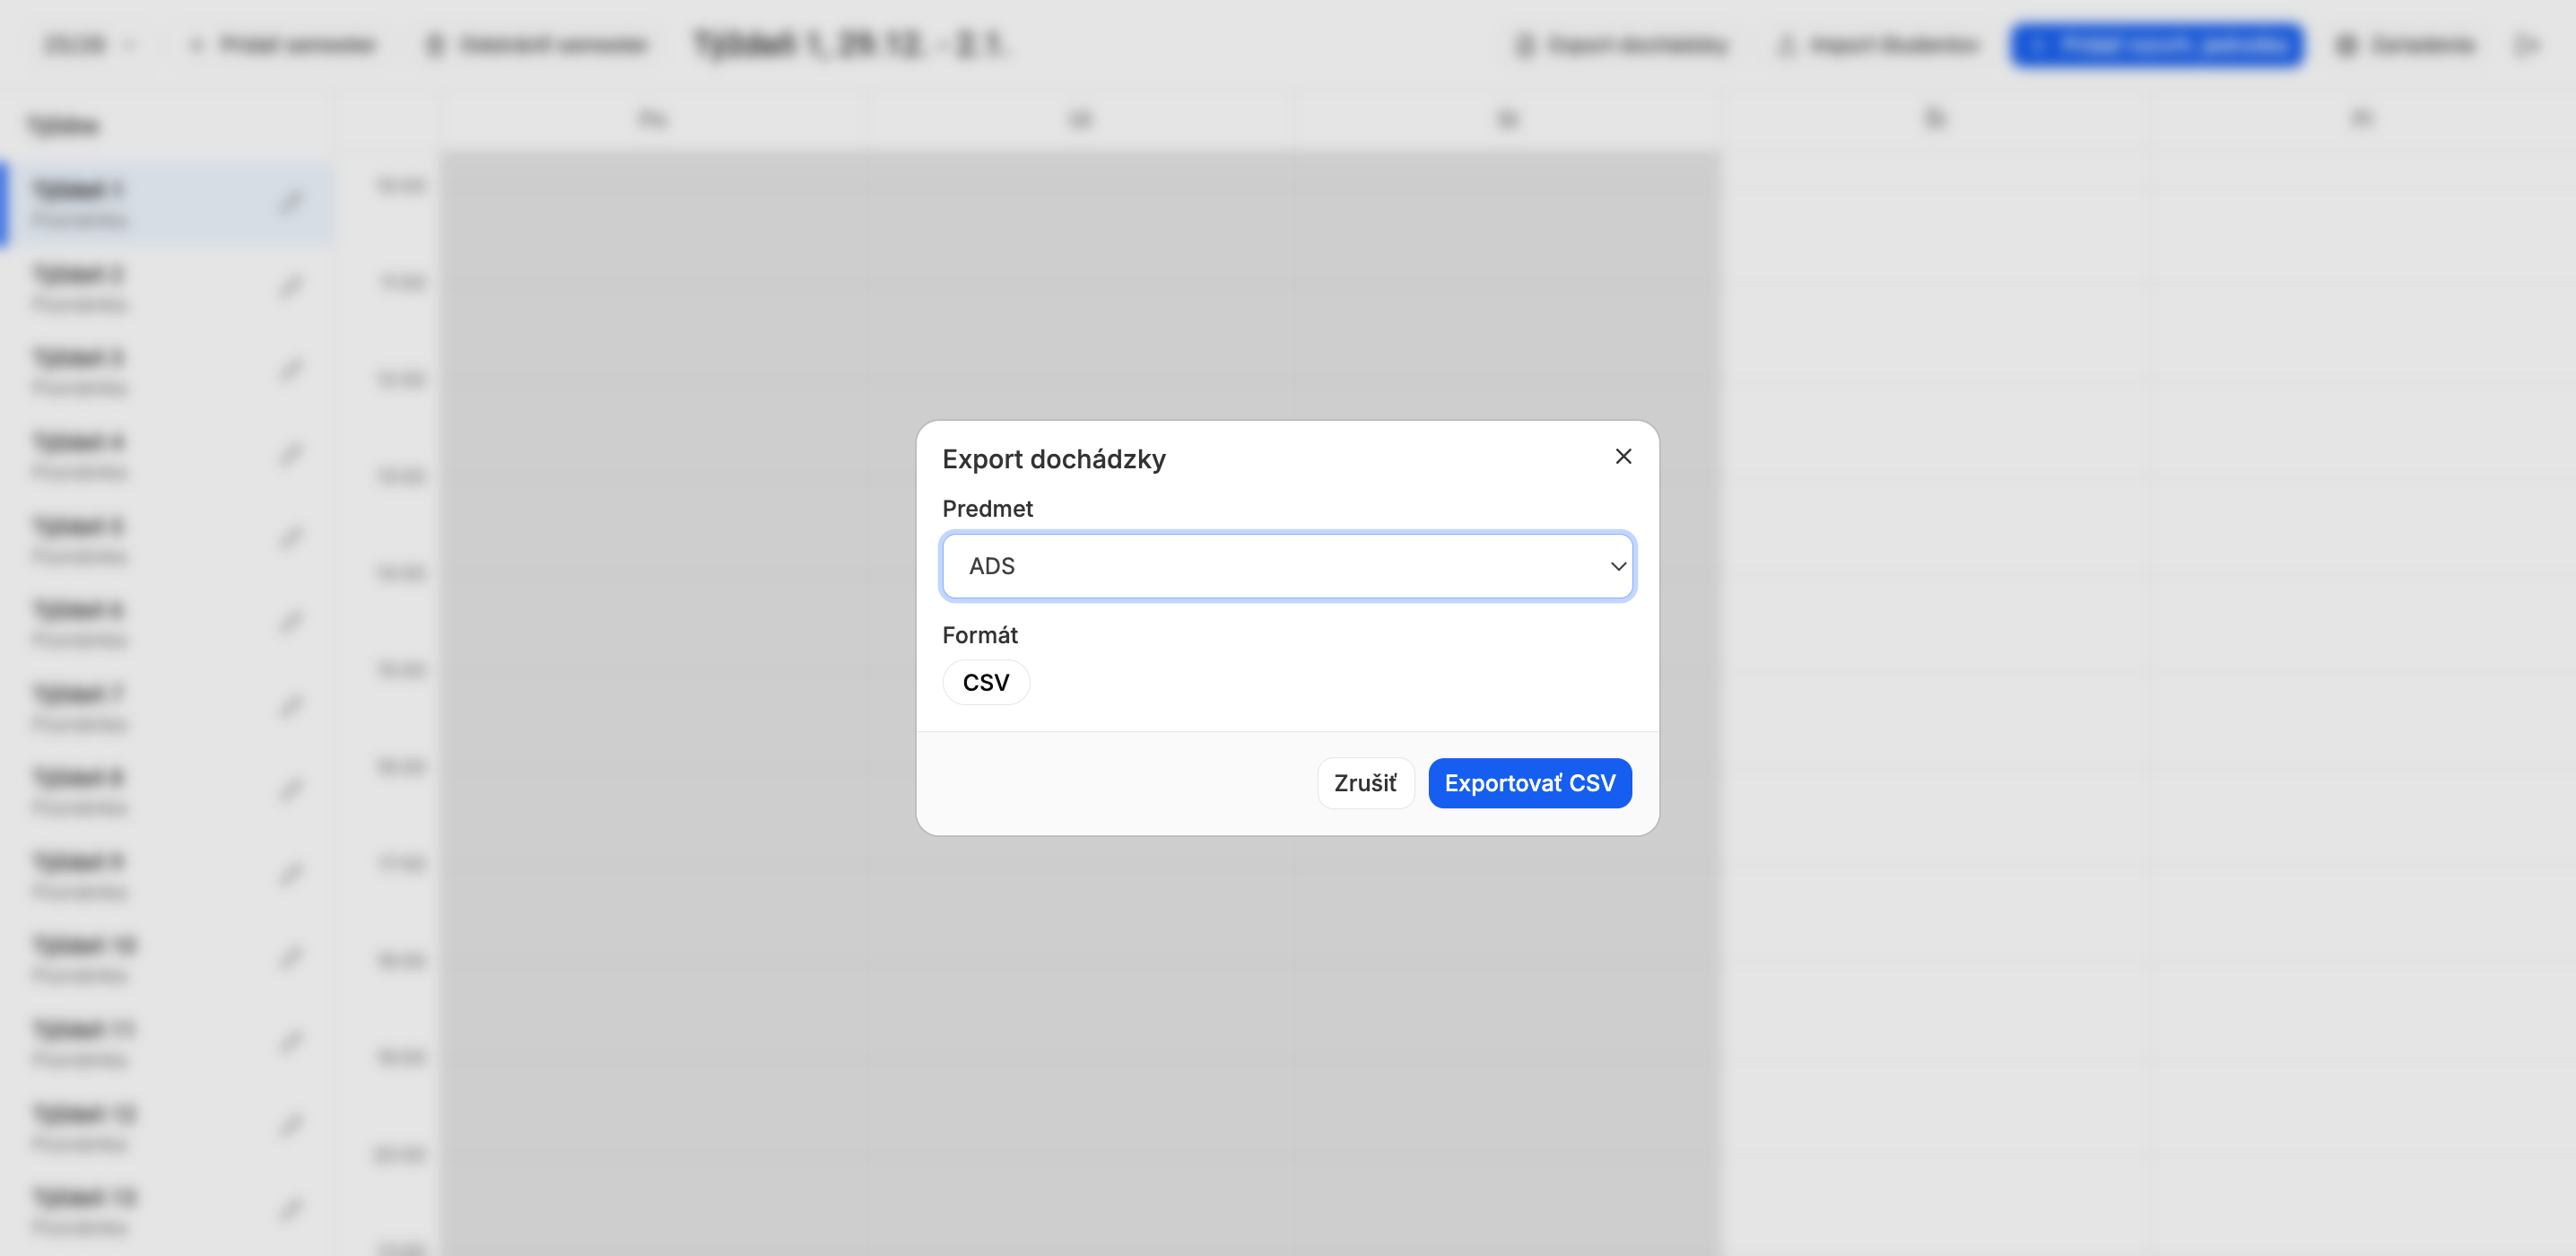
\includegraphics[width=0.72\textwidth]{figures/12-teacher-export-attendance.png}
    \caption{Dialóg na export dochádzky}
\end{figure}

Detail udalosti je implementovaný ako bočný panel. Zobrazuje predmet, typ hodiny, dátum, čas, opakovanie a zoznam študentov. Pri každom študentovi možno meniť stav dochádzky na hodnoty \texttt{Prítomný}, \texttt{Neprítomný}, \texttt{Náhrada} alebo \texttt{Ospravedlnený}.

\begin{figure}[!ht]
    \centering
    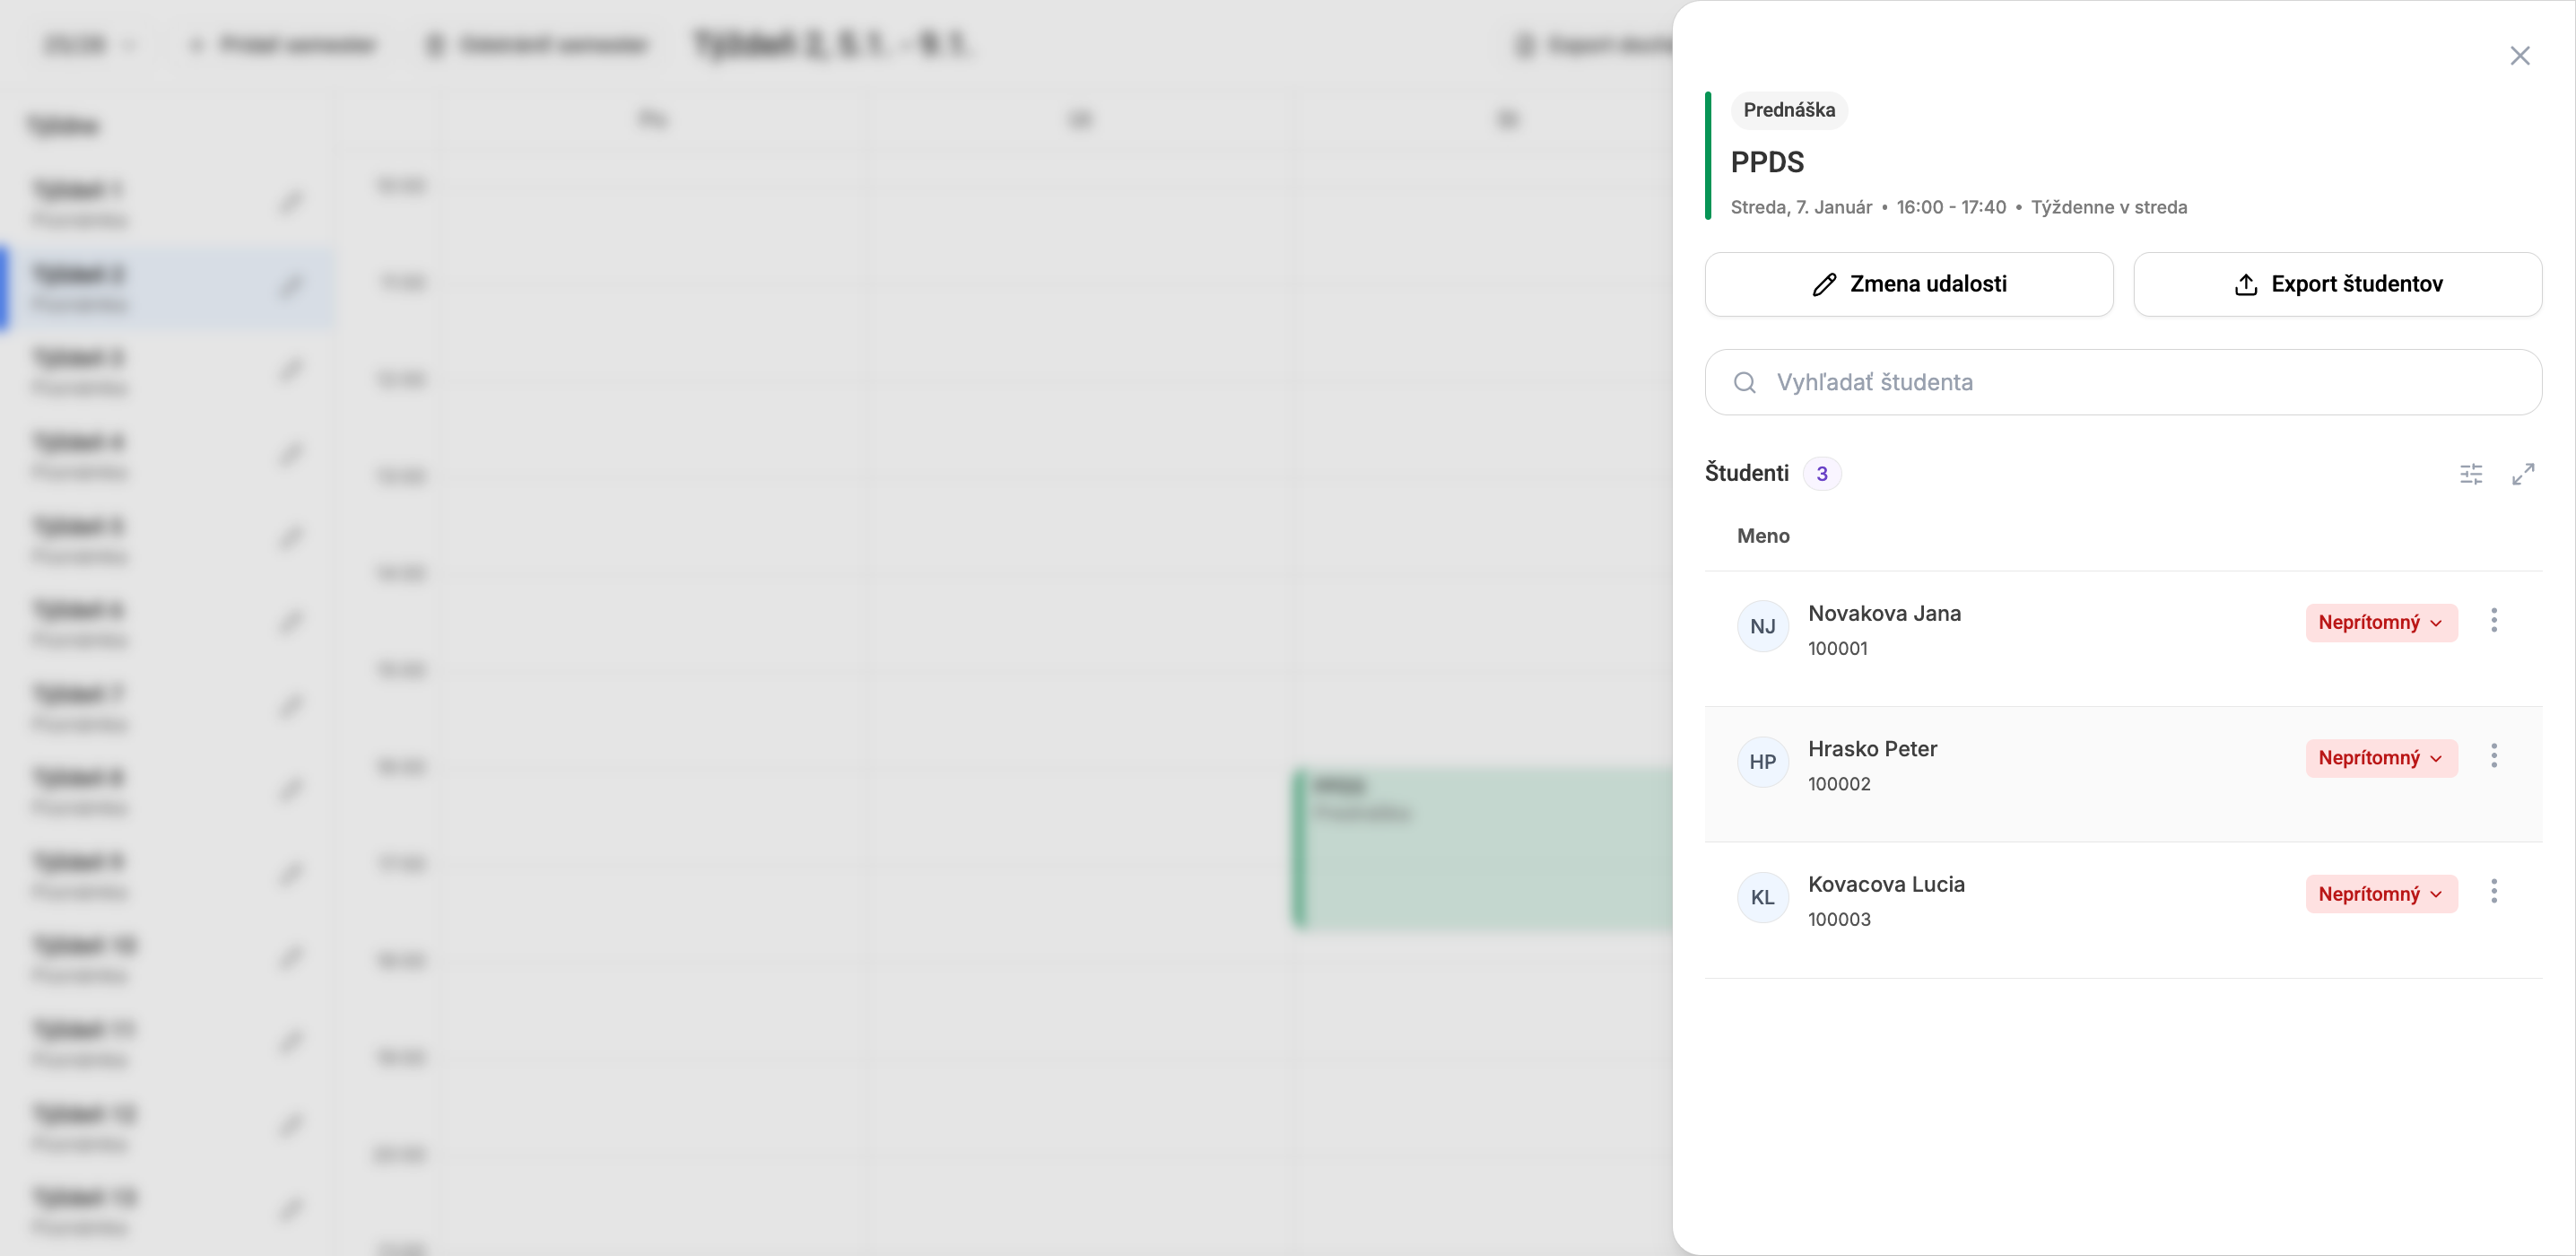
\includegraphics[width=0.9\textwidth]{figures/14-teacher-event-panel.png}
    \caption{Bočný panel detailu udalosti a dochádzky}
\end{figure}

Zmena stavu sa ukladá priamo po výbere novej hodnoty. Frontend zároveň podporuje priebežné obnovovanie dochádzky v pravidelných intervaloch. Tento mechanizmus je dôležitý najmä pri hodinách, kde sa prítomnosť aktualizuje na základe skenov z hardvérovej čítačky.

Prehľad predmetu je dostupný v rozšírenom zobrazení, kde sú študenti zobrazení v riadkoch a týždne v stĺpcoch. Takéto zobrazenie umožňuje rýchlo skontrolovať dochádzku za celý semester a vykonať hromadnejšiu orientáciu v stave predmetu.

\begin{figure}[!ht]
    \centering
    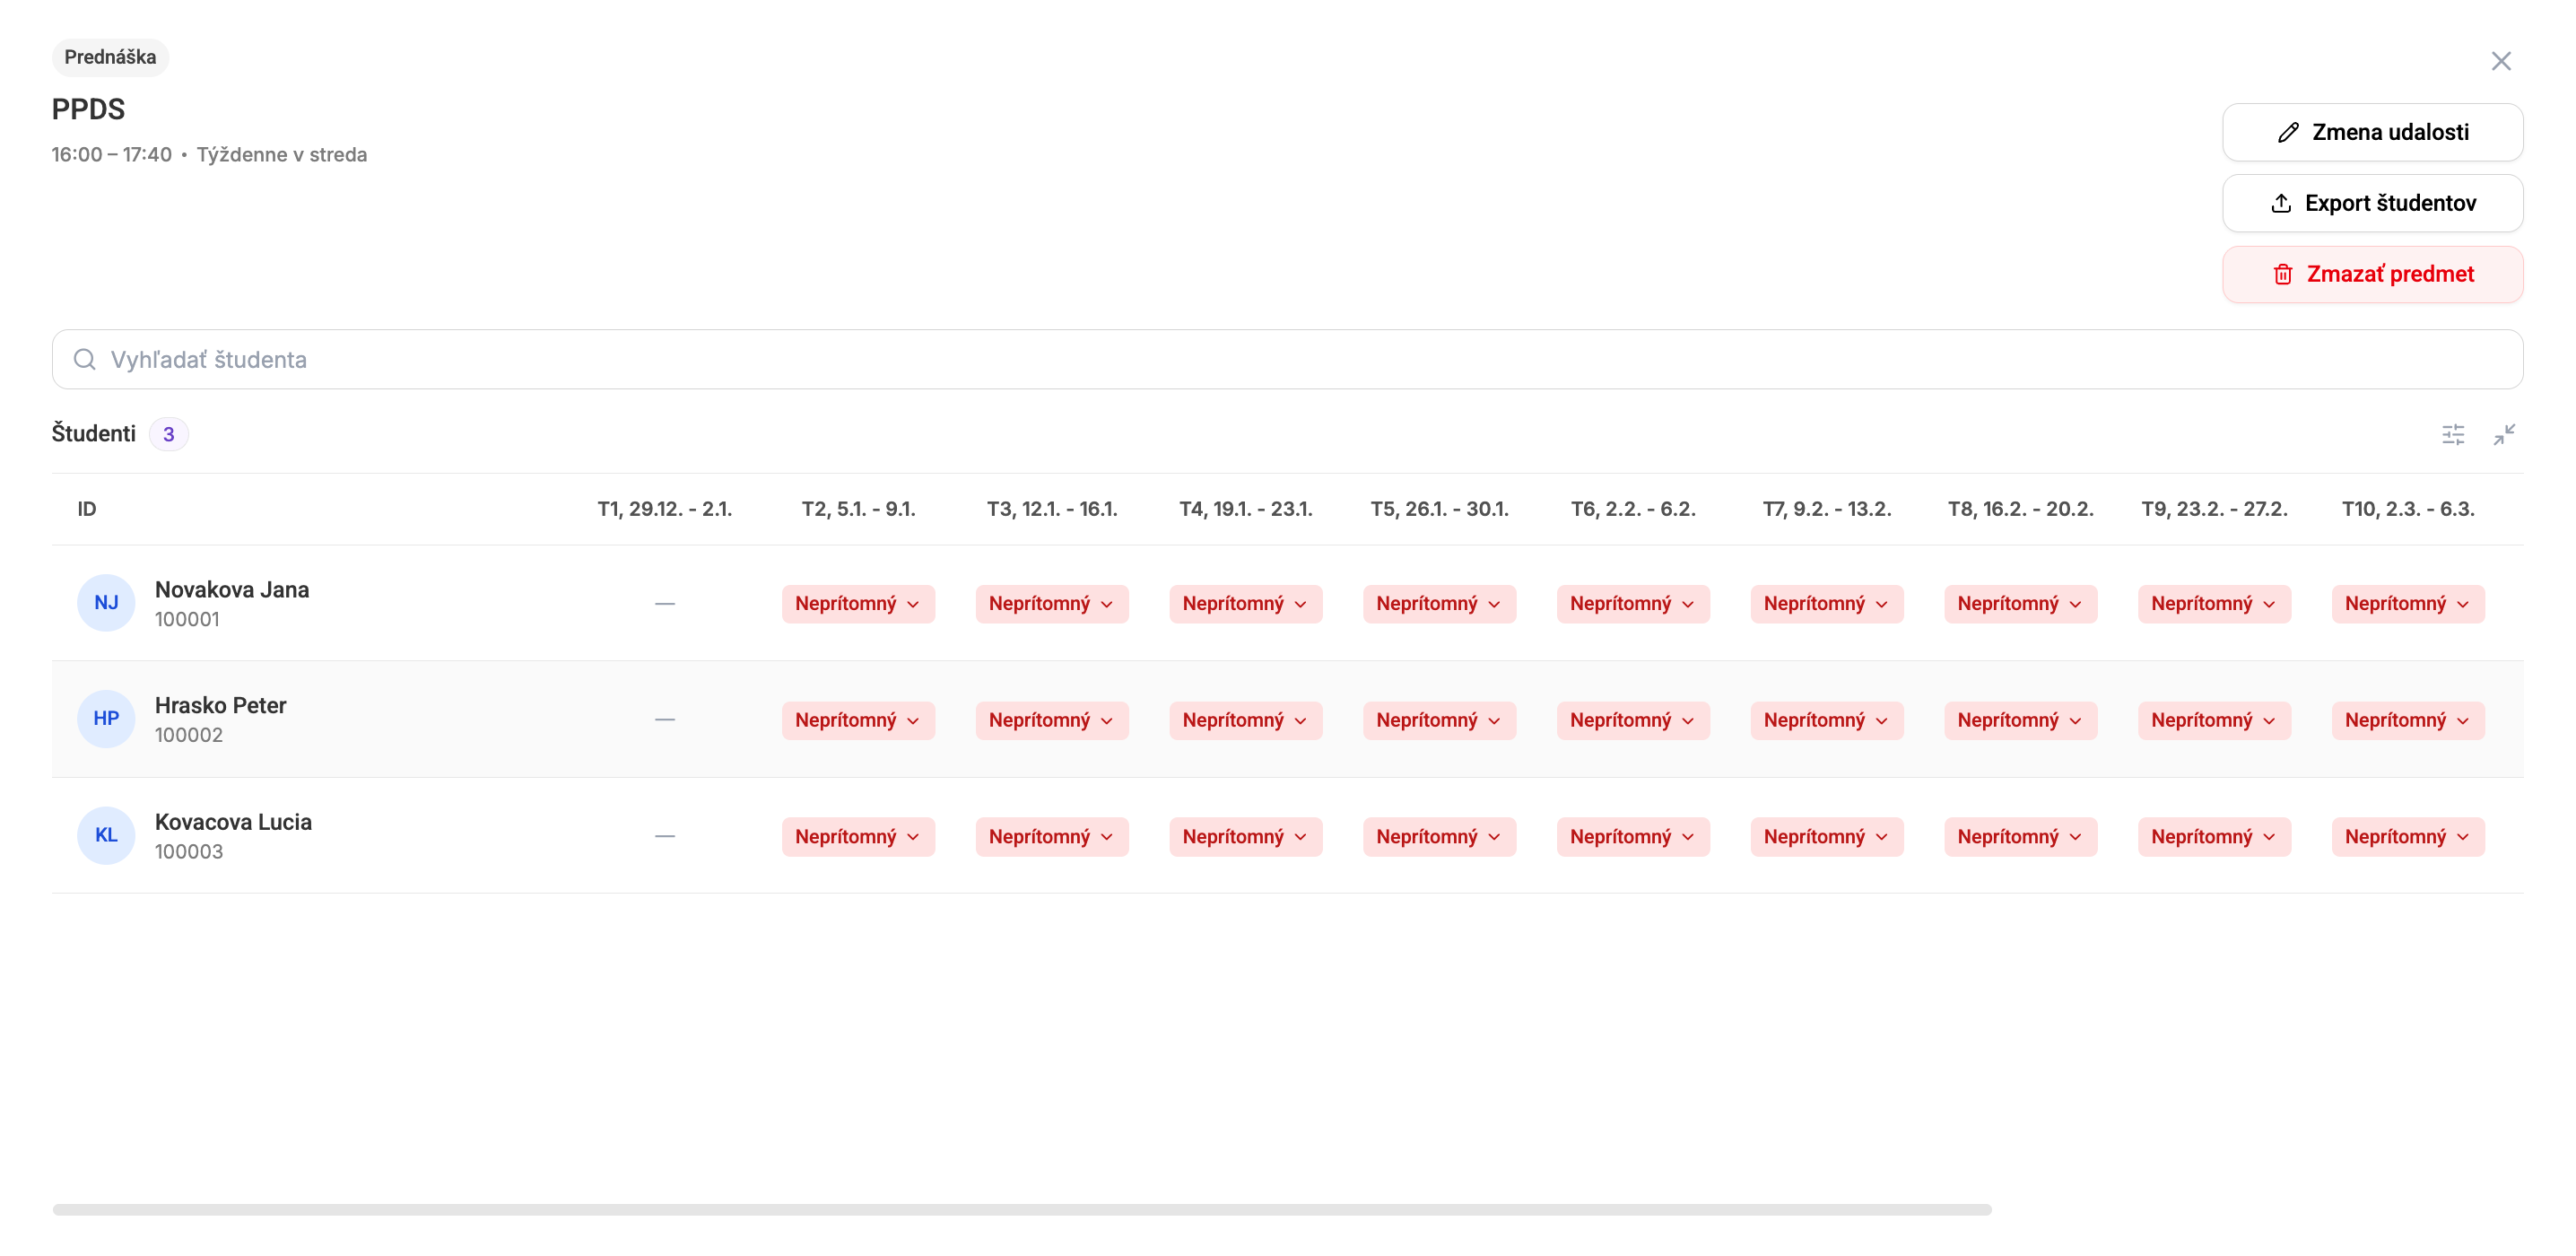
\includegraphics[width=0.95\textwidth]{figures/17-teacher-subject-overview.png}
    \caption{Rozšírený prehľad dochádzky predmetu naprieč semestrom}
\end{figure}

\section{Správa zariadení vyučujúceho}
\label{sec:frontend-teacher-hardware}

Okrem práce s rozvrhom a dochádzkou má vyučujúci k dispozícii aj obrazovku na správu vlastných zariadení. Táto časť slúži na párovanie čítačky s účtom vyučujúceho a na základnú kontrolu jej stavu.

\begin{figure}[!ht]
    \centering
    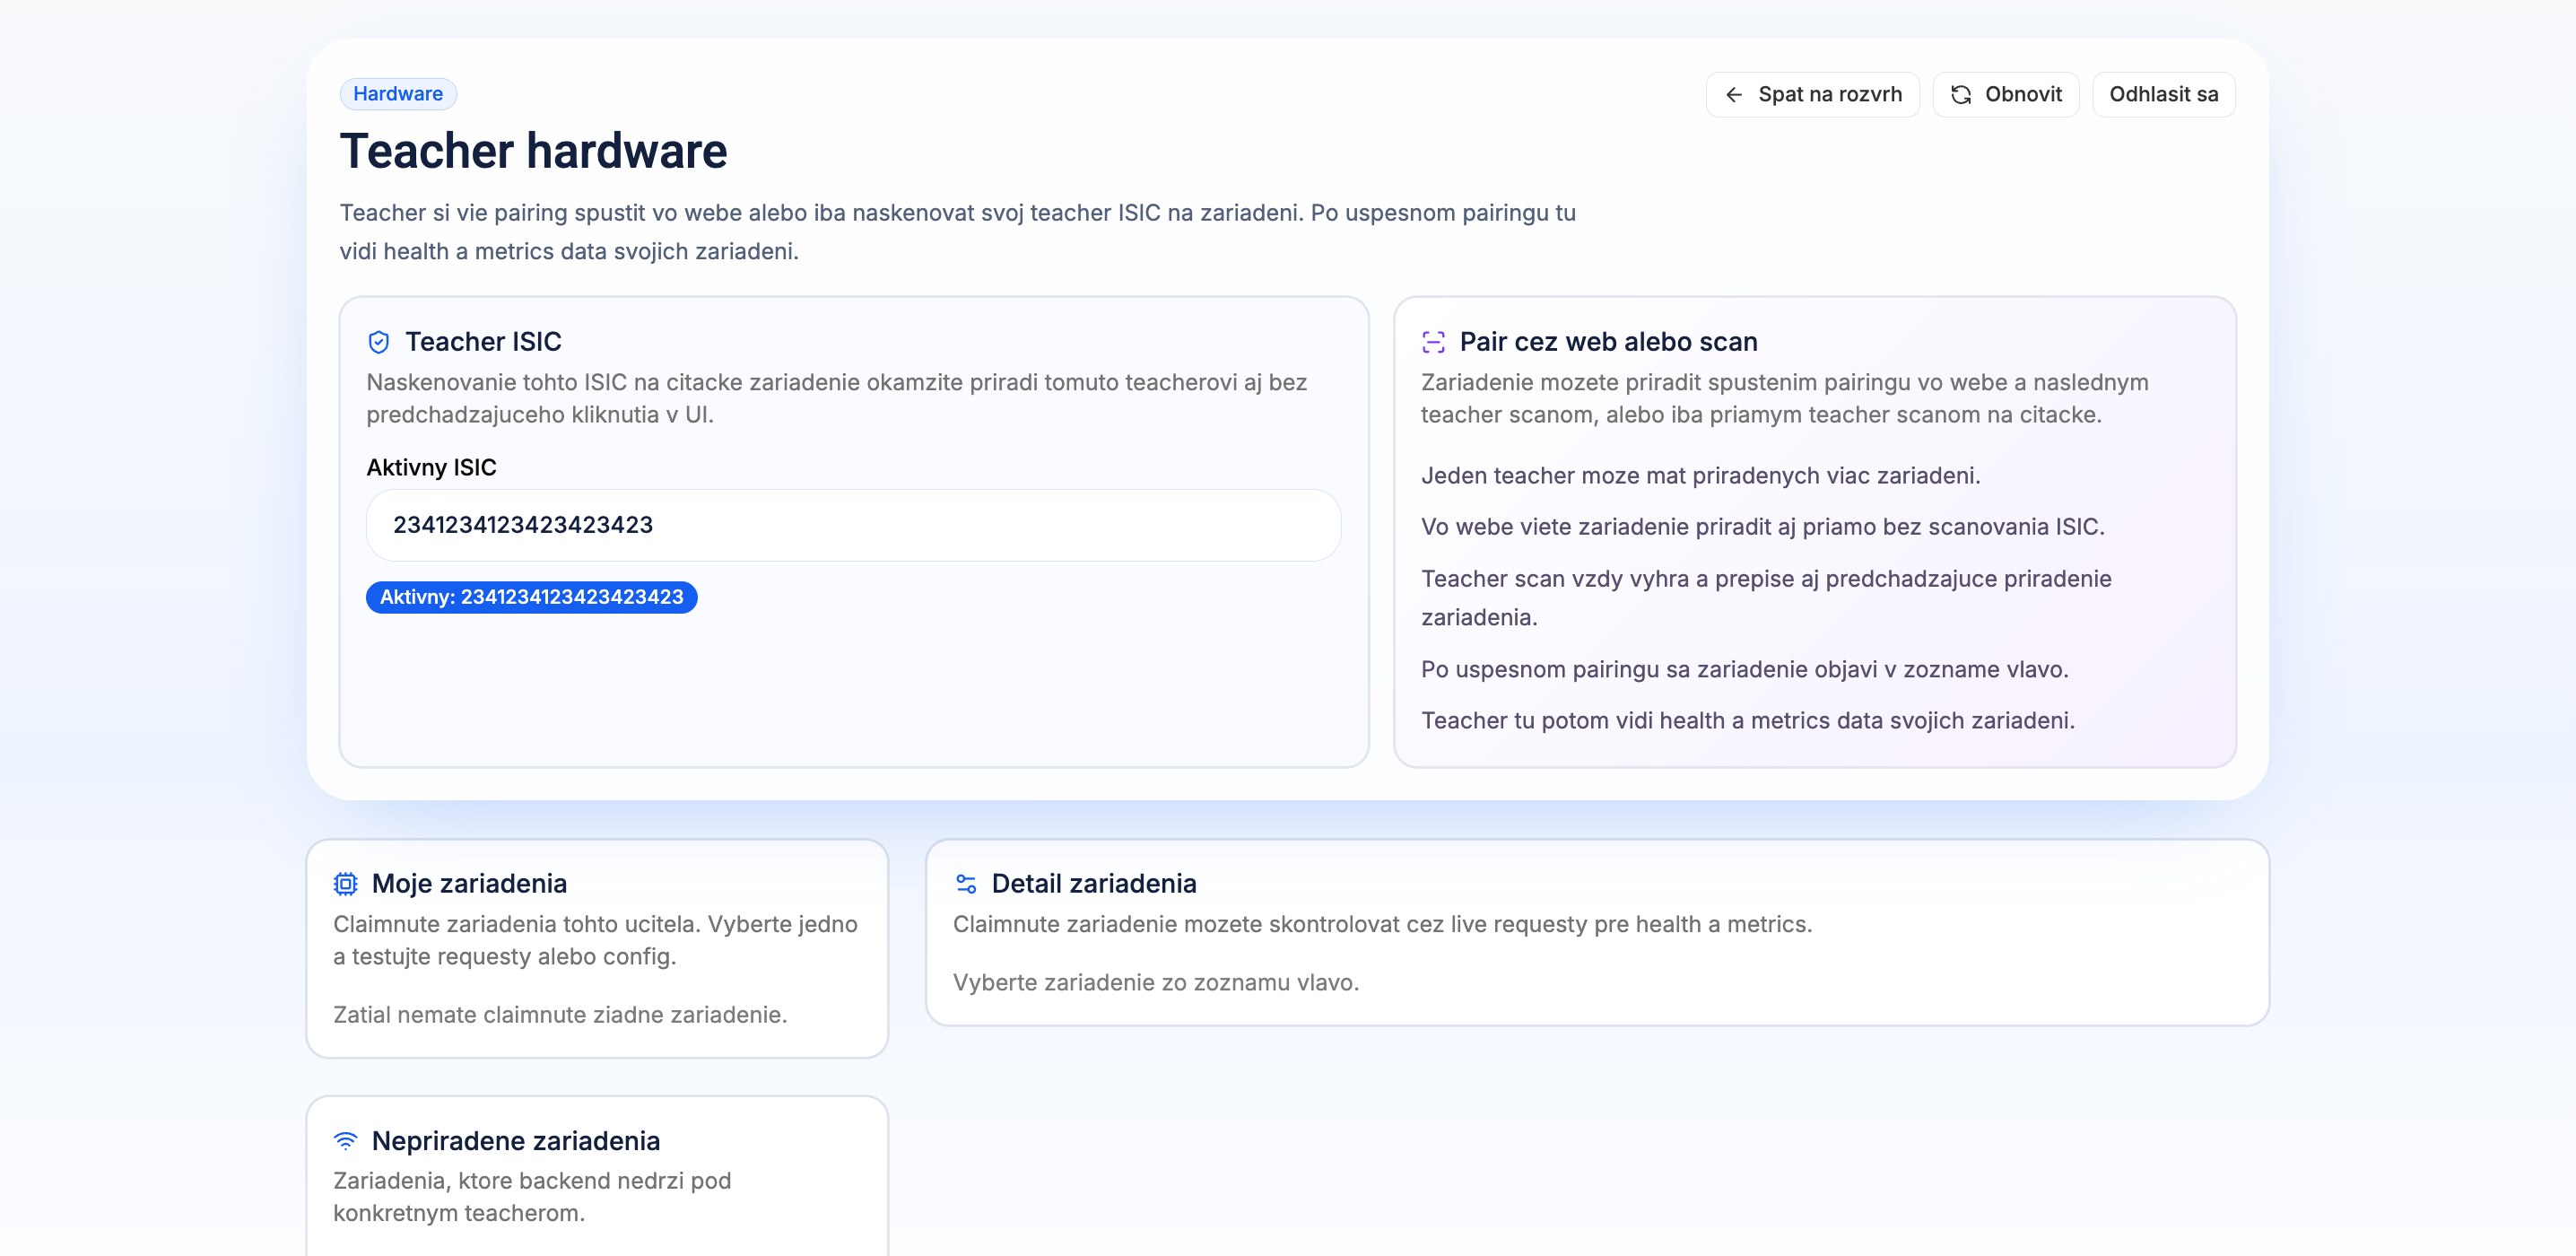
\includegraphics[width=0.92\textwidth]{figures/18-teacher-hardware.png}
    \caption{Hardvérová obrazovka vyučujúceho}
\end{figure}

Zariadenie možno priradiť dvoma spôsobmi. Prvým je spustenie párovania vo webovej aplikácii a následné naskenovanie teacher ISIC na čítačke. Druhým je priame naskenovanie karty bez predchádzajúceho kliknutia vo webovom rozhraní. Po úspešnom párovaní sa zariadenie zobrazí v zozname priradených čítačiek a frontend umožní zobraziť health údaje a metriky podobne ako v administrátorskej časti.

Súčasťou hardvérovej správy je aj podpora aktualizácie firmvéru zariadení. Frontend umožňuje nahrať OTA balík vo formáte \texttt{.zip}, skontrolovať jeho verziu a cieľovú platformu a následne pripraviť publikovanie firmvéru do vybraných zariadení. Tento postup je vhodný pri priebežnom nasadzovaní nových verzií firmvéru bez potreby fyzického zásahu do zariadenia.

\begin{figure}[!ht]
    \centering
    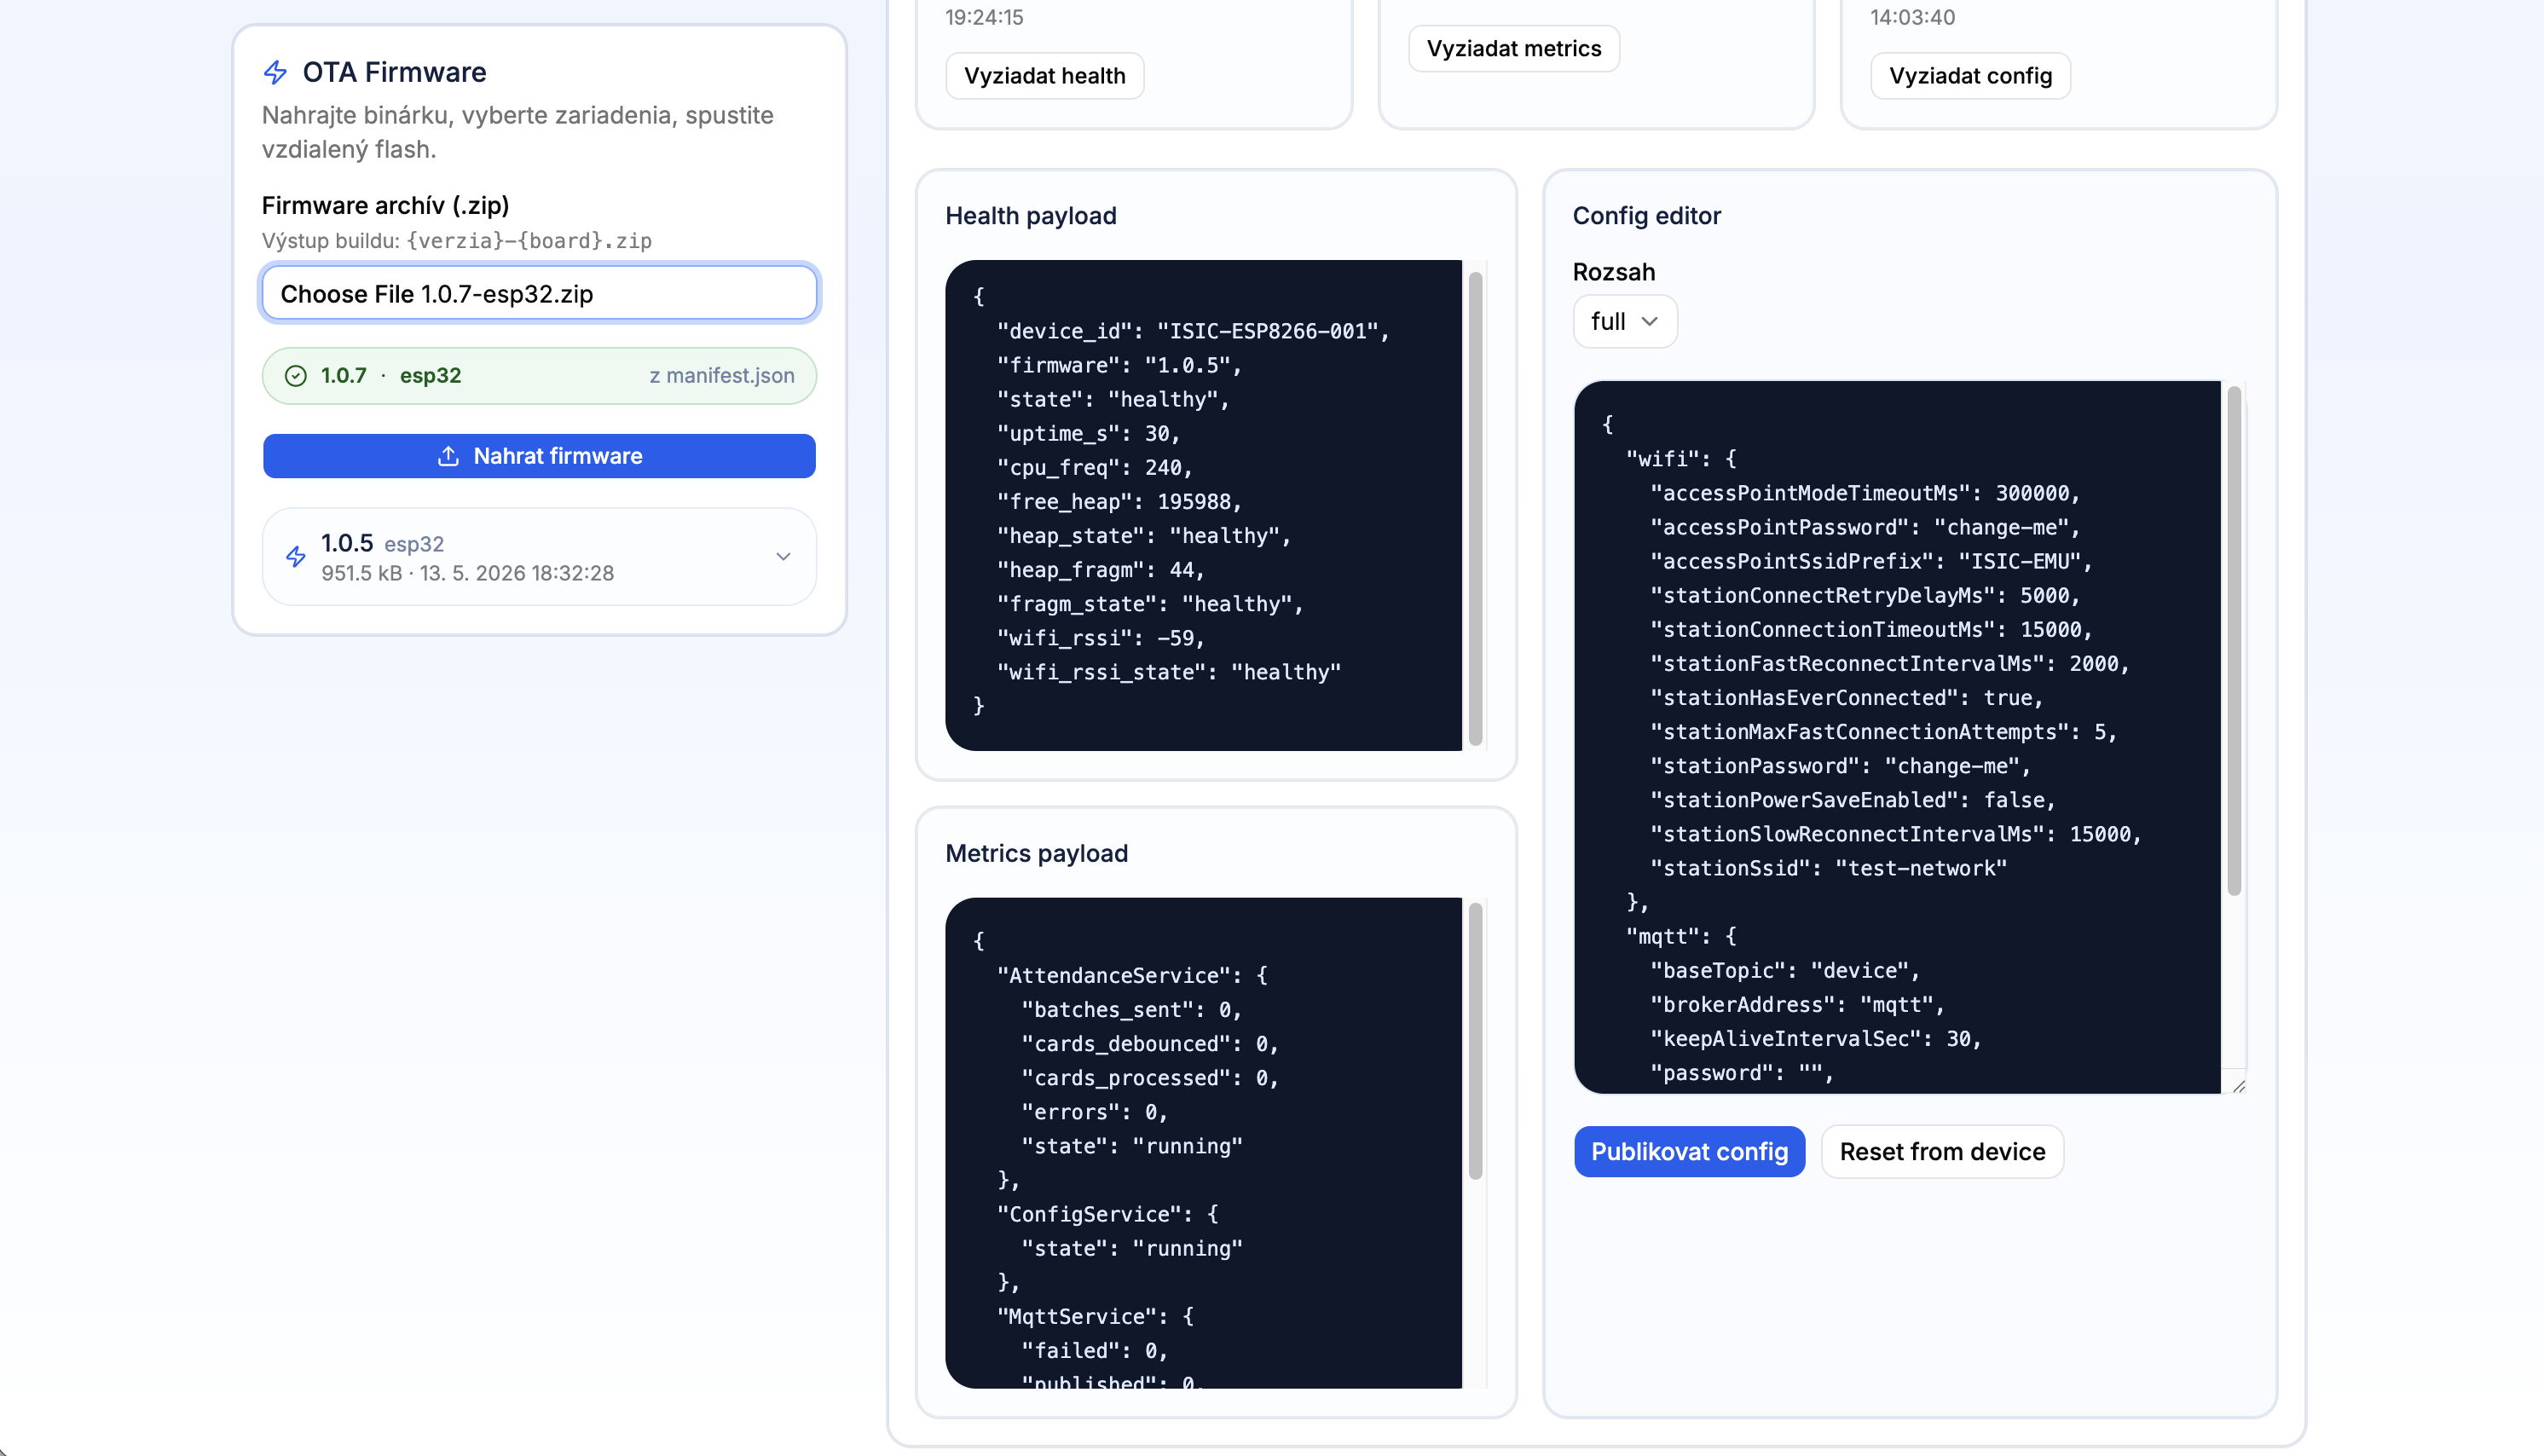
\includegraphics[width=0.72\textwidth]{figures/ota.png}
    \caption{Rozhranie na nahratie OTA firmvéru}
\end{figure}

Po nahratí firmvérového archívu môže používateľ otvoriť dialóg vzdialeného flashovania. V tomto dialógu vyberie konkrétne online zariadenia, na ktoré sa má nová verzia nasadiť.

\begin{figure}[!ht]
    \centering
    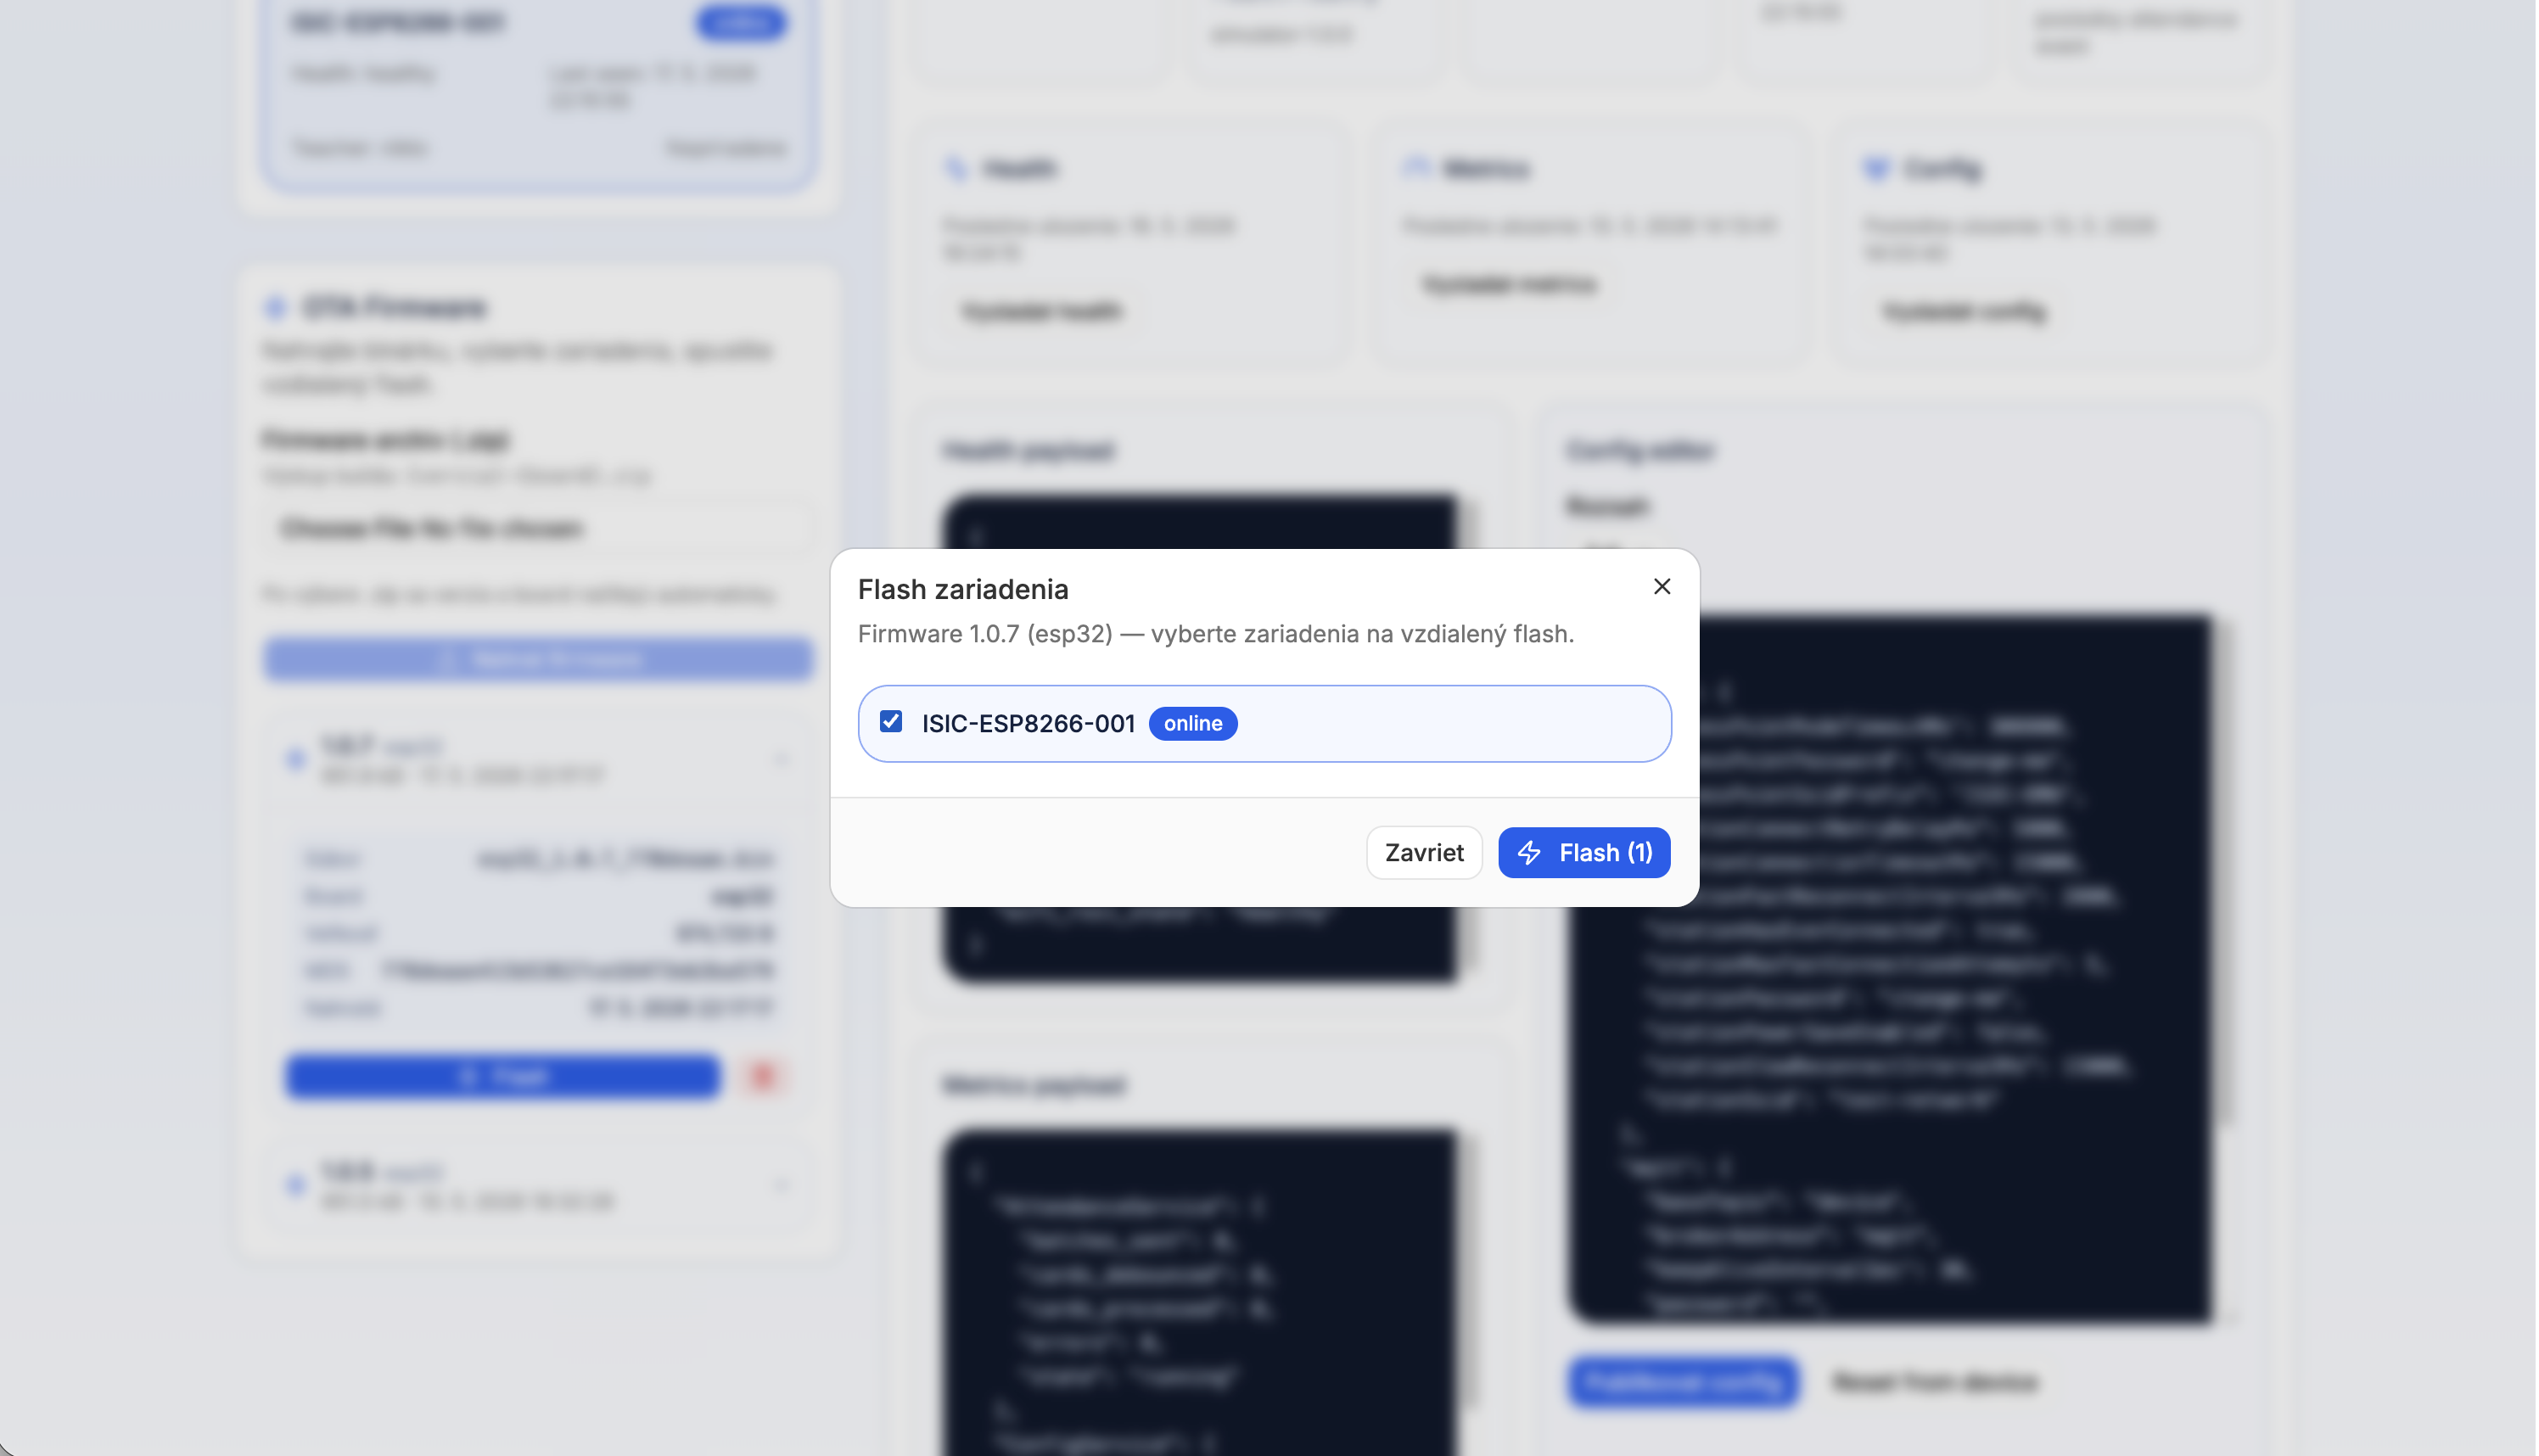
\includegraphics[width=0.72\textwidth]{figures/flash.png}
    \caption{Dialóg vzdialeného flashovania zariadenia}
\end{figure}

\section{Zhrnutie implementácie frontendu}
\label{sec:frontend-summary}

Frontendová časť systému \textit{ISIC Attendance} poskytuje jednotné webové rozhranie pre administrátora aj vyučujúceho. Zabezpečuje prihlasovanie, správu semestrov, kalendára, študentov, dochádzky aj hardvérových zariadení a pritom komunikuje s backendom cez typovo kontrolované REST API.

Architektúra založená na Reacte, TypeScripte a modulárnom rozdelení na feature časti umožňuje udržiavať prehľadný kód a postupne rozširovať funkcionalitu systému. Dôležitou vlastnosťou frontendu je aj priebežná aktualizácia dochádzky a dôraz na jednoduché formulárové rozhranie, ktoré uľahčuje každodennú prácu so systémom.
